%% Thesis template:
%% Final edits by Jussi Kangasharju and Pirjo Moen
%% This file is modified by Veli Mäkinen from HY_fysiikka_LuKtemplate.tex authored by Roope Halonen ja Tomi Vainio.
%% Some text is also inherited from engl_malli.tex by Kutvonen, Erkiö, Mäkelä, Verkamo, Kurhila, and Nykänen.

%%%%%
% Information about the compilation errors
%%%%%

% LaTeX Font Warning: Font shape `T1/lmr/m/scit' undefined
% (Font)              using `T1/lmr/m/scsl' instead on input line 160.
% This is safe to ignore:
% https://tex.stackexchange.com/questions/555332/latex-warning-after-update-miktex-font-shape-t1-lmr-m-scit-undefined-fontu

%%%%%
% Document
%%%%%

% This silences the warning
% LaTeX Font Warning: Font shape `T1/lmr/m/scit' undefined
% (Font)              using `T1/lmr/m/scsl' instead
% https://tex.stackexchange.com/a/572817/214874
\RequirePackage{silence}
\WarningFilter{latexfont}{Font shape `T1/lmr/m/scit'}

% STEP 1: Choose oneside or twoside
\documentclass[english,twoside,openright]{UH_TCM_MSc}
%finnish,swedish

% \documentclass[a4paper]{report}
% The package inputenc is disabled when using LuaLaTeX or XeLaTex, as those are utf8-based by default.
% \usepackage[utf8]{inputenc}
\usepackage[T1]{fontenc}

\usepackage{amsfonts} % mathbb etc.
\usepackage{amsmath, amssymb} % For better math
\usepackage[titletoc]{appendix}
\usepackage{babel}
\usepackage[backend=biber,sorting=none]{biblatex}
\usepackage{blindtext}
\usepackage{bm} % bold symbols in math mode
\usepackage[footnotesize,bf]{caption} % For more control over figure captions
\usepackage{csquotes} % Prevents the warning "'babel/polyglossia' detected but 'csquotes' missing"
\usepackage[en-GB]{datetime2}
\usepackage{fancyhdr} % For nicer page headers
\usepackage{color, graphicx} % For pdf output and jpg/png graphics
\usepackage[plainpages=false]{hyperref} % For hyperlinks and pdf metadata
\usepackage{listings}
\usepackage{lmodern} % Font package
% \usepackage{nomencl}
\usepackage{placeins} % FloatBarrier
%\usepackage[square]{natbib} % For bibliography
\usepackage{textcomp} % Package for special symbols
\usepackage{tikz} % For making vector graphics (hard to learn but powerful)
\usepackage{titlesec}
\usepackage{todonotes}
%\usepackage{wrapfig} % For nice text-wrapping figures (use at own discretion)
\usepackage{xcolor}


% For fixing LaTeX Unicode errors
% \DeclareUnicodeCharacter{FE20}{WARNING}
% \DeclareUnicodeCharacter{FE21}{WARNING}

% Glossary
% \loadglsentries[main]{tex/glossary.tex}
% \makeglossaries

% Citations
\addbibresource{tex/references.bib}
% \hypersetup{hidelinks}

\onehalfspacing %line spacing
%\singlespacing
%\doublespacing

%\fussy
\sloppy % sloppy and fussy commands can be used to avoid overlong text lines

% STEP 2:
% Set up all the information for the title page and the abstract form.
% Replace parameters with your information.
% \title{Equations of state for phase transitions in the early universe}
% \title{Self-similar hydrodynamics of first-order phase transitions in the early universe}
% The name has to be updated in the following places
% - Here
% - Hypersetup pdf title (below)
% - tex/references.bib
% - Project readme
\title{The effect of sound speed on the gravitational wave spectrum of first order phase transitions in the early universe}
\author{Mika Mäki}
% The thesis year has to be updated also at:
% - tex/references.bib
% - Project readme
% The \today macro should not be used on arXiv.
% https://info.arxiv.org/help/faq/today.html
\date{18th December 2024}
\prof{Professor Mark Hindmarsh}
\censors{Professor Mark Hindmarsh}{Professor Kari Rummukainen}{}
\depositeplace{}
\additionalinformation{}

% \classification{\protect{\ \\
% \  TODO General and reference $\rightarrow$ Document types  $\rightarrow$ Surveys and overviews\  \\
% \  Applied computing  $\rightarrow$ Document management and text processing  $\rightarrow$ Document management $\rightarrow$ Text editing\\
% }}
% Commenting this out results in an "Undefined control sequence.\end@summary error" later.
\classification{}

% if you want to quote someone special. You can comment this line and there will be nothing on the document.
%\quoting{Bachelor's degrees make pretty good placemats if you get them laminated.}{Jeph Jacques}


% OPTIONAL STEP: Set up properties and metadata for the pdf file that pdfLaTeX makes.
% But you don't really need to do this unless you want to.
\hypersetup{
    %bookmarks=true,         % show bookmarks bar first?
    unicode=true,           % to show non-Latin characters in Acrobat’s bookmarks
    pdftoolbar=true,        % show Acrobat’s toolbar?
    pdfmenubar=true,        % show Acrobat’s menu?
    pdffitwindow=false,     % window fit to page when opened
    pdfstartview={FitH},    % fits the width of the page to the window
    pdftitle={The effect of sound speed on the gravitational wave spectrum of first order phase transitions in the early universe}, % title
    pdfauthor={Mika Mäki},           % author
    pdfsubject={},          % subject of the document
    pdfcreator={},          % creator of the document
    pdfproducer={pdfLaTeX}, % producer of the document
    pdfkeywords={phase transitions} {gravitational waves} {sound speed} {Sound Shell Model},
    pdfnewwindow=true,      % links in new window
    colorlinks=true,        % false: boxed links; true: colored links
    linkcolor=black,        % color of internal links
    citecolor=black,        % color of links to bibliography
    filecolor=magenta,      % color of file links
    urlcolor=cyan           % color of external links
}

% \bibliography{bibliography}

% Actual document starts here
\begin{document}

\maketitle

% STEP 3:
% Write your abstract (of course you really do this last).
% You can make several abstract pages (if you want it in different languages),
% but you should also then redefine some of the above parameters in the proper
% language as well, in between the abstract definitions.

\begin{abstract}
The Standard Model of particle physics has proven to be remarkably accurate in various collider experiments,
but lacks explanations for some observed phenomena such as baryon asymmetry: Why is there more matter than antimatter?
The extensions of the Standard Model provide possible solutions to these questions,
but the energy scales required to distinguish between them are difficult to achieve in colliders.
However, many of these extensions also result in cosmological phase transitions that have occurred early in the Big Bang during the electroweak symmetry breaking at around $10^{-11} \text{s}$ or earlier.

If these phase transitions have been of first order,
they have created a stochastic background of gravitational waves that can be directly observed today.
The Laser Interferometer Space Antenna (LISA) space probe will be launched in the 2030s to study gravitational waves and
to see whether such a stochastic background exists.
If we see a signal of cosmological origin,
we need to be able to deduce the parameters of the phase transition from the gravitational wave signal to understand the physics behind it.
To accomplish this, we need simulations of the gravitational wave spectra with various parameters.
One such important parameter is the sound speed $c_s$.

The vast majority of existing simulations have been based on the bag model equation of state,
which assumes the ultrarelativistic sound speed $c_s =\frac{1}{\sqrt{3}}$ for both phases.
This was also the case for the PTtools phase transition simulation framework developed by Hindmarsh et al.
In this thesis PTtools has been extended to include support for arbitrary equations of state and therefore for a temperature- and phase-dependent sound speed $c_s(T,\phi)$.
Since the sound speed is such an integral part of the hydrodynamic equations,
this required a nearly complete rewrite and significant extension of the code.
The code has also been sped up considerably by the use of the Numba JIT compiler, various other optimisations and parallelisation,
and made conformant to modern coding standards.

PTtools was tested with the constant sound speed model, in which the sound speed is a constant for each phase.
The sound speed was shown to have a significant effect on the resulting gravitational wave spectrum,
especially when changing the sound speed resulted in a change in the type of the solution.
This has laid the groundwork for simulating cosmological phase transitions with realistic equations of state based on the extensions of the Standard Model.
This will result in gravitational wave spectra that can be used in the LISA data analysis pipeline to search for the existence and parameters of a first-order phase transition in the early universe.

\end{abstract}

% Place ToC
% \tableofcontents
\mytableofcontents

% This seems to be broken, but it's necessary for the correct page numbering.
\mynomenclature
% \makenomenclature

\clearpage
\listoffigures
\clearpage
\listoftables
\clearpage

% Remove this before submitting the thesis!
% \listoftodos
% \clearpage

% \chapter*{Abstract}
% The Standard Model of particle physics has proven to be remarkably accurate in various collider experiments,
but lacks explanations for some observed phenomena such as baryon asymmetry: Why is there more matter than antimatter?
The extensions of the Standard Model provide possible solutions to these questions,
but the energy scales required to distinguish between them are difficult to achieve in colliders.
However, many of these extensions also result in cosmological phase transitions that have occurred early in the Big Bang during the electroweak symmetry breaking at around $10^{-11} \text{s}$ or earlier.

If these phase transitions have been of first order,
they have created a stochastic background of gravitational waves that can be directly observed today.
The Laser Interferometer Space Antenna (LISA) space probe will be launched in the 2030s to study gravitational waves and
to see whether such a stochastic background exists.
If we see a signal of cosmological origin,
we need to be able to deduce the parameters of the phase transition from the gravitational wave signal to understand the physics behind it.
To accomplish this, we need simulations of the gravitational wave spectra with various parameters.
One such important parameter is the sound speed $c_s$.

The vast majority of existing simulations have been based on the bag model equation of state,
which assumes the ultrarelativistic sound speed $c_s =\frac{1}{\sqrt{3}}$ for both phases.
This was also the case for the PTtools phase transition simulation framework developed by Hindmarsh et al.
In this thesis PTtools has been extended to include support for arbitrary equations of state and therefore for a temperature- and phase-dependent sound speed $c_s(T,\phi)$.
Since the sound speed is such an integral part of the hydrodynamic equations,
this required a nearly complete rewrite and significant extension of the code.
The code has also been sped up considerably by the use of the Numba JIT compiler, various other optimisations and parallelisation,
and made conformant to modern coding standards.

PTtools was tested with the constant sound speed model, in which the sound speed is a constant for each phase.
The sound speed was shown to have a significant effect on the resulting gravitational wave spectrum,
especially when changing the sound speed resulted in a change in the type of the solution.
This has laid the groundwork for simulating cosmological phase transitions with realistic equations of state based on the extensions of the Standard Model.
This will result in gravitational wave spectra that can be used in the LISA data analysis pipeline to search for the existence and parameters of a first-order phase transition in the early universe.


\chapter{Introduction}
\label{ch:introduction}
Raise the interest of the reader!

Tip for style: discuss the same things from another point of view (in the light of the results) in the conclusion.
-> Binds the thesis together.

\begin{itemize}
    \item Background for the choice of theme
    \item A discussion of the research question or thesis statement
    \item A schematic outline of the thesis
\end{itemize}

Research question: how to simulate the gravitational spectra caused by different equations of state with PTtools?

This thesis is available \href{https://gitlab.com/AgenttiX/msc-thesis2}{online}.
TODO license with Creative Commons Attribution 4.0 International, as is done for the lecture notes.

Matter-antimatter asymmetry \cite{lecture_notes}

LISA in the 2030s.


\chapter{Phase transitions in the early universe}
\label{ch:pt}
\section{Todo notes}

Equations of state
\begin{itemize}
    \item Bag model \cite[eq. 7.33]{lecture_notes}
    \item Assumptions on speed of sound and constant parameters
    \item Giese's paper \cite{giese_2020}
    \item Enqvist, old paper \cite{enqvist_nucleation_1992}
\end{itemize}

Employment?
- "things that need to be done"
-> suitable for public dissemination
- write some short description,
    - ArXiv paper

2 papers by Giese, second one is more complete
Paper 1 \cite{giese_2020}
Paper 2 \cite{giese_2021}

TODO: understand these
\begin{itemize}
    \item Relativistic hydrodynamics from the review article (aka. lecture notes) \cite{lecture_notes}
    \item Reviews from other people (not just Hindmarsh)
    \item Article by Mazumdar \& White, especially section 7: relativistic combustion \cite{mazumdar_review_2019}
    \item The sound shell model paper
    \item Really understand what's going on! Compute with pen \& paper etc.
    \item Relativistic hydrodynamics
    \begin{itemize}
        \item The book by Luciano Rezzolla \& Olindo Zanotti \cite{rezzolla_relativistic_2013}
        \item Read the part I (some 300 pages at first)
        \item Contains more than necessary for the thesis
    \end{itemize}
    \item The phase transition section should have plenty of content before Christmas
    \item Enqvist's paper
    \begin{itemize}
        \item Good background: connects the equations of state to particle physics
        \item -> What kinds of equations of state would a particle theory produce
        \item Assumes ultrarelativisticity, which is no longer necessary due to the improvement of computational tools
    \end{itemize}
    \item Ultimately the equation of state can be derived from the "Thermal effective potential".
    \item Chemical potential is zero, as there is no conserved particle number.
    \item J-function, fB, lecture eq. 2.19 etc.
    \begin{itemize}
        \item These will be our first equation of state.
    \end{itemize}
\end{itemize}

"My job is to give the GWs the right energy-momentum tensor"

\section{Basics}
Electroweak symmetry breaking at $10^{-11}$ s, $100$ -- $1000$ GeV.
First-order phase transition
-> bubbles just below the critical temperature
-> gravitational waves

Standard model has a crossover, but many extensions first-order.

Matter-antimatter asymmetry -> net baryon number
(But isn't B an accidental symmetry, whereas B-L is a fundamental one?
How does this correspond to the neutrino content of the universe?)
\cite{lecture_notes}

The gravitational wave spectrum can be calculated from a few thermodynamic properties of ultrarelativistic matter, which can be computed from quantum field theory.
These parameters can be measured by LISA.



\section{Relativistic hydrodynamics}
% Statistical mechanics \cite{huang_statistical_1987}
% \cite{schroeder_thermal_2000}
% \cite[ch. 4]{lecture_notes}
% According to Hindmarsh it's OK to have references on the level of individual chapters and equations.

Our system of interest is an ultrarelativistic plasma.
This means, that the energy of the particles is much higher than their rest mass.
Therefore there is sufficient energy for new particles to be created,
and similarly existing particles will annihilate all the time.
Treating this kind of a system as a classical fluid is not sufficient,
and we need the mathematical machinery of general relativity.

In general relativity the matter and energy content of space are described by the \textbf{energy-momentum tensor} $T^{\mu \nu}$, also known as the stress-energy tensor.
In Minkowski space in Cartesian coordinates it's given as
\cites[eq. 4.17]{rasanen_gr_2022}[fig. 3.3]{rezzolla_relativistic_2013}
\begin{equation}
T_{\mu \nu} =
\begin{bmatrix}
e & -q_1 & -q_2 & -q_3 \\
-q_1 & p + \Pi_{11} & \Pi_{12} & \Pi_{13} \\
-q_2 & \Pi_{12} & p + \Pi_{22} & \Pi_{23} \\
-q_3 & \Pi_{13} & \Pi_{23} & p + \Pi_{33}
\end{bmatrix},
\end{equation}
where $q$ is the energy flux or momentum density and $\Pi_{\mu \nu}$ is known as the anisotropic stress, anisotropic pressure or momentum flux.
\href{https://physics.stackexchange.com/a/412067/298623}{In our case we assume the energy-matter content to be an ideal fluid in thermal equilibrium.}
There is no energy transfer to or from the fluid, and therefore
$\forall j=1,2,3: \quad T^{0j} = 0$.
As the fluid has no viscosity, it does not experience any shear stress, and therefore
$\forall i,j=1,2,3, \quad i \neq j: \quad T^{ij} = 0$.
This does not depend on the reference frame, so the tensor is diagonal in all reference frames.
Therefore $T^{ij} = p \delta^{ij}$.
These are satisfied only by the tensor $T^{00}=e, T^{jj}=p, \forall i \neq j: T^{ij}=0$.
It should be noted that the
\href{https://en.wikipedia.org/wiki/Einstein_notation}{Einstein notation} will be used for the indices throughout the thesis.
Greek indices are used for four-vectors and latin indices for three-vectors.
% The Einstein notation is absolute basics for theoretical physicists, but unfortunately the study programme of many of my applied/technical physicists friends doesn't involve it, so I'm mentioning it explicitly here so that they can google it.
This
\href{https://en.wikipedia.org/wiki/Stress\%E2\%80\%93energy\_tensor\#Stress\%E2\%80\%93energy\_of\_a\_fluid\_in\_equilibrium}{\textbf{energy-momentum tensor of an ideal fluid}}
can be broken in two components as
\cites[eq. 5.11, 5.23]{lecture_notes}[eq. 4.12]{rasanen_gr_2022}
% [eq. 3]{giese_2020}[eq. 4]{giese_2021}
\begin{align}
T^{\mu \nu}_f
&= (e+p) u^\mu u^\nu + p g^{\mu \nu}
\label{eq:ep_tensor} \\
&= w u^\mu u^\nu + p g^{\mu \nu}.
\end{align}

We are assuming the background space-time to be constant, and therefore the total \textbf{energy-momentum is conserved}.
In the language of general relativity this is
\begin{equation}
\nabla_\mu T^{\mu\nu} = 0.
\label{eq:ep_conservation}
\end{equation}
Here $\nabla_\mu$ is the covariant derivative, which in Minkowki space in Cartesian coordinates reduces to the partial derivative $\partial_\mu$.
To expand this equation in a way consistent with \cite[ch. 3.3]{rezzolla_relativistic_2013} we need to define the projection tensor
\cite[eq. 3.9]{rezzolla_relativistic_2013}
\begin{equation}
h_{\mu\nu} \equiv g_{\mu\nu} + u_\mu u_\nu,
\label{eq:projection_tensor}
\end{equation}
and the expansion scalar
\cite[eq. 3.13]{rezzolla_relativistic_2013}
\begin{equation}
\Theta \equiv h^{\mu\nu} \nabla_\nu u_\mu = \nabla_\mu u^\mu.
\end{equation}
Inserting these to \eqref{eq:ep_conservation} results in
% The specific enthalpy is not a meaningful quantity for an ultrarelativistic fluid, and is therefore not used here.
\begin{equation}
\nabla_\mu T^{\mu \lambda} = u^\lambda u^\mu \nabla_\mu (e+p) + (e+p) u^\mu \nabla_\mu u^\lambda + (e+p) \Theta u^\lambda + g^{\lambda\mu} \nabla_\mu p.
\end{equation}
\todo{Should enthalpy be introduced before this? It would make the e+p terms simpler.}
Relativistic acceleration is defined as
\begin{equation}
a_\nu = u^\mu \nabla_\mu u_\nu.
\end{equation}
It is orthogonal to the velocity, and therefore
\begin{equation}
a^\mu u_\mu = 0.
\end{equation}
Projecting using \eqref{eq:ep_conservation} and using these we get
\cite[eq. 3.54]{rezzolla_relativistic_2013}
\begin{equation}
\bm{h} \cdot \bm{\nabla} \cdot \bm{T}
= h^\nu_\lambda \nabla_\mu T^{\mu \lambda}
= (e+p) u^\mu \nabla_\mu u^\nu + h^\nu_\lambda g^{\lambda\mu} \nabla_\mu p
= 0.
\end{equation}
It should be noted that \cite{rezzolla_relativistic_2013} uses the specific enthalpy $h$ in their form these equations, but it is not a meaningful quantity for an ultrarelativistic plasma and is therefore not used here.
Dividing by $e+p$ we get the \textbf{relativistic Euler equations}
\cite[eq. 3.55]{rezzolla_relativistic_2013}
\begin{equation}
u^\mu \nabla_\mu u_\nu + \frac{1}{e+p} h^\mu_\nu \nabla_\mu p = 0.
\end{equation}
Similarly we can project along the direction of velocity,
\begin{equation}
\bm{u} \cdot \bm{\nabla} \cdot \bm{T} = u_\lambda \nabla_\mu T^{\mu\lambda} = 0.
\end{equation}
This results in the \textbf{energy-conservation equation}
\cite[eq. 3.57]{rezzolla_relativistic_2013}
\begin{equation}
u^\mu \nabla_\mu e + (e+p) \Theta = 0.
\end{equation}

For a one-dimensional flow in Cartesian coordinates the energy-momentum conservation of \eqref{eq:ep_conservation} can also be rewritten as
\begin{align}
\partial_t \left[ (e+pv^2) \gamma^2 \right] + \partial_x \left[ (e+p) \gamma^2 v \right] &= 0,
\label{eq:ep_conservation_1d_1} \\
\partial_t \left[ (e+p) \gamma^2 v \right] + \partial_x \left[ (ev^2 + p) \gamma^2 \right] &= 0
\label{eq:ep_conservation_1d_2}
\end{align}
by simply inserting \eqref{eq:ep_tensor} and using the normalisation of four-velocity $u_\mu u^\mu = -1$.
Let's then analyse a perturbation on a fluid that is at rest with $e_0, p_0$ and $v_0 = 0$.
To first order
\begin{equation}
e = e_0 + \delta e, \quad p=p_0 + \delta p, \quad v = v_0 + \delta v = \delta v.
\end{equation}
Substituting these into \eqref{eq:ep_conservation_1d_1} and \eqref{eq:ep_conservation_1d_2} and approximating to first order in the perturbation results in
\begin{align}
\partial_t (\delta e) + (e_0 + p_0) \partial_x (\delta v) = 0,
\label{eq:ep_conservation_rewritten_1} \\
\partial_t (\delta v) + \frac{1}{e_0 + p_0} \partial_x (\delta p) = 0.
\label{eq:ep_conservation_rewritten_2}
\end{align}
Taking the time derivative of \eqref{eq:ep_conservation_rewritten_1} and a space derivative of \eqref{eq:ep_conservation_rewritten_2}, we can combine the equations to the form
\begin{equation}
\partial_t^2 (\delta e) - \frac{\delta p}{\delta e} \partial_x^2(\delta e) = 0.
\end{equation}
This is the familiar wave equation, so the motion of the fluid has wave solutions that we call sound.
\cite[ch. 4.3]{rezzolla_relativistic_2013}
The speed of sound is then defined as
\cites[eq. 2.168]{rezzolla_relativistic_2013}[eq. 13]{giese_2020}[eq. 3]{giese_2021}
\begin{align}
c_s^2
&\equiv \frac{dp}{de} \\
&= \frac{dp/dT}{de/dT}
\end{align}
At the ultrarelativistic limit $e=3p$ and therefore $c_s^2=\frac{1}{3}$.
\todo{Write here why}

\iffalse
The
\href{https://en.wikipedia.org/wiki/Clausius\%E2\%80\%93Clapeyron_relation}{Clausius-Clapeyron relation} states that
% According to Hindmarsh it's OK to have hyperlinks to unofficial sources such as Wikipedia.
\cite[eq. 5.47, 5.48]{schroeder_thermal_2000}
\begin{equation}
\frac{dp}{dT} = \frac{L}{T \Delta V} = \frac{\Delta S}{\Delta V}.
\end{equation}
\fi

Proper discussion of relativistic fluids also requires various thermodynamic quantities.
\todo{Derive entropy density properly}
% Let us start from the thermodynamic identity of classical thermal physics

Perturbing around a constant $U$ (effectively setting $dU=0$) gives the entropy density
\todo{Is this the correct explanation?}
\cite[p. 23]{lecture_notes}
\begin{equation}
s \equiv \frac{dS}{dV} = \frac{dp}{dT}.
\label{eq:entropy_density}
\end{equation}

Useful formulas for other thermodynamic quantities can be obtained from the thermodynamic identity of classical thermal physics.
\cites[eq. 2.136]{rezzolla_relativistic_2013}[eq. 3.68]{schroeder_thermal_2000}
\begin{equation}
dU = TdS - pdV + \mu dN,
\label{eq:thermodynamic_identity}
\end{equation}
where $U$ is internal energy, $T$ is temperature, $p$ is pressure, $V$ is volume, $\mu$ is chemical potential and $N$ is the number of particles.
The fluids in our case are ultrarelativistic, and therefore effectively $T >> \mu$,
and we can neglect $dN$.

Inserting \eqref{eq:entropy_density} to \eqref{eq:thermodynamic_identity} gives the \textbf{energy density}
\begin{equation}
e \equiv \frac{dU}{dV} = T \frac{\partial p}{\partial T} - p.
\end{equation}
This in turn can be inserted to the definition of enthalpy
\cite[eq. 1.51]{schroeder_thermal_2000}
\begin{equation}
H \equiv E + pV
\end{equation}
to get the \textbf{enthalpy density}
\begin{align}
w
&\equiv \frac{dH}{dV} \\
&= e+p \\
&= T \frac{\partial p}{\partial T} \\
&= Ts.
\end{align}
\iffalse
Additionally we need to define the \textbf{specific enthalpy} \cite[eq. 2.141]{rezzolla_relativistic_2013}
\begin{equation}
h = \frac{e+p}{\rho},
\label{eq:specific_enthalpy}
\end{equation}
where $\rho$ is the rest-mass density, and the \textbf{entropy current}
% Rest-mass density is defined in eq. 2.123
\fi
Additionally we need to define the \textbf{entropy current}
\cite[p. 23]{lecture_notes}
\begin{equation}
S^\mu \equiv su^\mu.
\end{equation}



\section{Field-fluid system}
Based on \cite{moore_pt_1995}.

In the electroweak phase transition the fluid is coupled to a scalar field with the energy-momentum tensor
\cites[eq. 2.9]{hindmarsh_gw_pt_2019}
\begin{equation}
T_\phi^{\mu \nu}
= \partial^\mu \partial^\nu \phi
- g^{\mu \nu} \left(\frac{1}{2} (\partial \phi)^2 + V_0 (\phi) \right)
\end{equation}

The total energy-momentum is conserved,
\cite[eq. 5.17]{lecture_notes}
\begin{equation}
\partial_\mu T^{\mu \nu} = \partial_\mu (T_f^{\mu \nu} + T_\phi^{\mu \nu}) = 0.
\end{equation}



\section{Relativistic combustion}
This chapter of the lecture notes is largely based on the references
% According to Hindmarsh, abbreviating "references" as "refs" is OK in the thesis.
\cites{hindmarsh_gw_pt_2019}{espinosa_energy_2010}.
\todo{Add more content from \cite[ch. 6]{mazumdar_review_2019}.}

If the wall velocity is constant, \eqref{eq:ep_conservation} also holds in the wall frame.
Therefore for a wall moving in the z-direction
\cite[eq. 7]{espinosa_energy_2010}
\begin{equation}
\partial_z T^{zz} = \partial_z T^{z0} = 0.
\end{equation}
Inserting the definition of $T$ from \eqref{eq:ep_tensor} results in the bubble wall junction conditions
\cites[eq. 7.22]{lecture_notes}[eq. B.2-3]{hindmarsh_gw_pt_2019}
% This is almost trivial.
\begin{align}
w_- \tilde{\gamma}_-^2 \tilde{v}_- &= w_+ \tilde{\gamma}_+^2 \tilde{v}_+, \\
w_- \tilde{\gamma}_-^2 \tilde{v}_-^2 + p_- &= w_+ \tilde{\gamma}_+^2 \tilde{v}_+^2 + p_+
\end{align}
These can be rearranged as
\cites[eq. 7.32]{lecture_notes}[eq. 6-7]{giese_2020}
\todo{How to prove this step? My attempts of manual proof have failed.}
\begin{align}
\tilde{v}_+ \tilde{v}_- = \frac{p_+ - p_-}{e_+ - e_-} \\
\frac{\tilde{v}_+}{\tilde{v}_-} = \frac{e_- + p_+}{e_+ + p_-}
\label{eq:junction_ep}
\end{align}
Further simplification of these requires additional definitions
that we will now introduce.

The trace of the energy-momentum tensor of \eqref{eq:ep_tensor} is
\begin{align}
\text{tr} (T^{\mu \nu})
&= T^\mu_\mu \\
&= g_{\mu \nu} T^{\mu \nu} \\
&=3p - e
\end{align}
We can quantify its difference from zero with the trace anomaly
\cites[eq. 7.24]{lecture_notes}[eq. 28]{giese_2020}
\begin{equation}
\theta = \frac{1}{4}(e-3p).
\end{equation}
The definition of the trace anomaly varies by a factor of $\frac{1}{4}$ depending on the source as a matter of convention.
The difference of the trace anomalies just ahead and behind of the wall is denoted as
\begin{align}
\Delta \theta
&\equiv \theta_+ - \theta_- \\
&= \theta_s - \theta_b
\end{align}
With this we can define the transition strength
\begin{equation}
\alpha_+ = \frac{4 \Delta \theta}{3 w_+}.
\end{equation}
We can also define the enthalpy ratio
\begin{equation}
r = \frac{w_+}{w_-}.
\end{equation}
With these definitions the junction conditions of \eqref{eq:junction_ep} can be simplified as
\begin{equation}
\tilde{v}_+ \tilde{v}_- = \frac{1-(1-3\alpha_+)r}{3-3(1+\alpha_+)r},
\quad
\frac{\tilde{v}_+}{\tilde{v}_-} = \frac{3+(1-3\alpha_+)r}{1+3(1+\alpha_+)r}.
\end{equation}
% If a superlative is without a noun, there is no "the".
This is easiest to prove in the reverse direction.
To further get expressions for $\tilde{v}_+$ and $\tilde{v}_-$ that are independent of $r$, we can extract $r$ from both equations and mark those as equal, resulting in the equation
\begin{equation}
\left( \frac{1}{\tilde{v}_-} + 3 \tilde{v}_- \right) v_+ - 3(1+\alpha_+)v_+^2 = \alpha_+ - 1.
\end{equation}
% Derivation: Mathematica Eliminate[] and a bit of simplification.
This is of second order in both $\tilde{v}_+$ and $\tilde{v}_-$ and can be solved as \cite[eq. B.6, B.7]{hindmarsh_gw_pt_2019}
\begin{align}
\tilde{v}_+ &= \frac{1}{2(1+\alpha_+)}\left[ \left(\frac{1}{3\tilde{v}_-}+\tilde{v}_-\right) \pm \sqrt{\left(\frac{1}{3\tilde{v}_-} - \tilde{v}_- \right)^2 + 4\alpha_+^2 + \frac{8}{3} \alpha_+} \right]
\label{eq:v_tilde_plus}
\\
\tilde{v}_- &= \frac{1}{2} \left[ \left( (1+\alpha_+)\tilde{v}_+ + \frac{1-3\alpha_+}{3\tilde{v}_+} \right) \pm \sqrt{\left((1+\alpha_+)\tilde{v}_+ + \frac{1-3\alpha_+}{3\tilde{v}_+} \right)^2 - \frac{4}{3}} \right)
\label{eq:v_tilde_minus}
\end{align}
Both of these are basic second-order solutions, but in \eqref{eq:v_tilde_plus} the discriminant has been simplified.



We can obtain useful continuity equations from the conservation of energy-momentum.
We start by defining two vectors, the fluid 4-velocity
\begin{equation}
u^\mu = \gamma(-1, \overrightarrow{v})^\mu
\end{equation}
and its orthonormal vector
\begin{equation}
\bar{u}^\mu = \gamma(-v, \frac{\overrightarrow{v}}{v})^\mu.
\end{equation}
These form an orthonormal basis.
It should be noted, that for orthonormal vectors
\begin{align}
% Note that the lecture notes use ubar here.
u_\mu u^\mu &= -1, \\
u_\mu \bar{u}^\mu &= 0.
\end{align}
By projecting the conservation equation to this basis we get
\begin{align}
0 = u_\mu \partial_\nu T^{\mu \nu} = -\partial_\mu (w u^\mu) + u^\mu \partial_\mu p \\
0 = \bar{u} \partial_\nu T^{\mu \nu} = w \bar{u}^\nu u^\mu \partial_\mu u_\nu + \bar{u}^\mu \partial_\mu p
\end{align}

Dimensionless coordinate
\begin{equation}
\xi = \frac{r}{t}
\end{equation}

Hydrodynamic equations, aka. continuity equations
\todo{Todo: Derive these}
\cites[eq. 7.30-7.31]{lecture_notes}[eq. 5]{giese_2021}
\begin{align}
\frac{dv}{d\xi} &= \frac{2v(1-v^2)}{\xi(1-v\xi)} \left( \frac{\mu(\xi,v)^2}{c_s^2} - 1 \right)^{-1} \\
\frac{dw}{d\xi} &= w \left( 1 + \frac{1}{c_s^2} \right) \gamma^2 \mu(\xi,v) \frac{dv}{d\xi}
\end{align}

It should be highlighted that everything in this chapter is independent of the equation of state introduced in the next chapter.


\section{The bag model}
The equation of state is the function $p(T)$ or $p(w)$ that characterises the behaviour of the fluid as a function of temperature $T$ or enthalpy $w$.
One of the simplest equations of state is the bag model, where
\cites[eq. 7.33]{lecture_notes}[eq. 8-9]{giese_2020}
\begin{align}
p_s &= a_s T^4 - V_s
\label{eq:bag_ps} \\
p_b &= a_b T^4,
\label{eq:bag_pb}
\end{align}
where $a_s$, $a_b$ and $V_s$ are positive constants with $a_s > a_b$.
s=symmetric, b=broken.

In this model the speed of sound simplifies as
\begin{equation}
c_s^2 = \frac{dp}{de} = 1/3,
\end{equation}
This corresponds to assuming the bth phases to be ultrarelativistic.

The name of the bag model originates from quantum chromodynamics (QCD), where it's used to describe the proton as a bag of quarks.
\todo{check this}


\section{More complex models}
The bag model includes severe approximations, and for realistic simulations a more complex model is needed.
The primary parameters for these models are
\begin{itemize}
    \item The phase transition parameters: percolation temperature, phase transition duration
    \item Bubble wall velocity
    \item Fraction of energy that is converted into fluid motion: $\kappa$
    \item Numerical prefactor from lattice simulations
\end{itemize}

Speed of sound may not be ultrarelativistic, especially in the broken phase.

\subsection{The constant sound speed model}
The constant sound speed model, also known as the $\mu, \nu$ model, expands the bag model by allowing a change in the speed of sound of the broken phase.
\cites[eq. 15]{giese_2021}[eq. 38]{giese_2020}
\begin{align}
p_s &= \frac{1}{3} a_+ T^\mu - \epsilon \\
p_b &= \frac{1}{3} a_- T^\nu \\
e_s &= a_+ T^\mu + \epsilon \\
e_b &= \frac{1}{3} a_- (\nu - 1) T^\nu
\end{align}
The parameters $a_+$ and $a_-$ are proportional to the number of relativistic degrees of freedom in the symmetric and broken phases, and $\epsilon$ is the temperature-independent vacuum energy that is released in the phase transition.
The parameters $\mu$ and $\nu$ are determined by the sound speeds in the symmetric and broken phases:
\cites[eq. 16]{giese_2021}[eq. 39]{giese_2020}
\begin{align}
\mu = 1 + \frac{1}{c_{s,s}^2}, \\
\nu = 1 + \frac{1}{c_{s,b}^2}.
\end{align}
\footnote{Please note that there is a typo in \cite[eq. 15]{giese_2021}. There the 4 should be a $\mu$.}

\subsection{Model with cubic thermal effects}
Free energy
\todo{Where does this come from? How to extract the thermal effects?}
\cite[eq. 45]{giese_2020}
\begin{align}
\begin{split}
\textsc{F}(\phi, T) =
&- \frac{a_+}{3} T^4 \\
&+ \lambda \left( \phi^4 - 2E\phi^3 T + \phi^2 \left( E^2 T_\text{cr}^2 + c \left( T^2 - T_\text{cr}^2 \right) \right) \right) \\
&+ \frac{\lambda}{4} \left( c - E^2 \right)^2 T_\text{cr}^4
\end{split}
\end{align}

The minimum of the field potential is given by
\cite[eq. 46]{giese_2020}
\begin{equation}
\phi_\text{min} = \frac{3}{4} ET + \sqrt{\frac{T^2}{2}(\frac{9}{8}E^2 - c) - \frac{T_\text{cr}^2}{2} (E^2 - c)}
\end{equation}

\subsection{Model with a two-step phase transition}
Two scalar fields and two symmetry breakings. Examples: electroweak symmetry, $\mathbb{Z}_2$ symmetry.
Cubic term is neglected.
Pressures are of the form
\cite[eq. 47-48]{giese_2020}
\begin{align}
p_s(T) = \frac{1}{3}a_+ T^4 + (b_+ - c_+ T^2)^2 - b_-^2 \\
p_b(T) = \frac{1}{3}a_+ T^4 + (b_- - c_-T^2)^2 - b_-^2
\end{align}
Compare these to the \eqref{eq:bag_ps}, \eqref{eq:bag_pb}.



\section{Types of solutions}
\missingfigure{Figure of the three different types of relativistic combustion. \cite[fig. 14]{lecture_notes}}

Subsonic deflagrations

Detonations

Supersonic deflagrations (hybrids)


\section{Energy redistribution}
Efficiency factor $\kappa$, which is the fraction of energy that is converted into fluid motion.
\begin{equation}
\kappa = \frac{3}{\xi_w^3 \Delta \theta} \int d\xi \xi^2 w \gamma^2 v^2
\end{equation}
From solving the hydrodynamic equations of state of a single expanding bubble.

Kinetic energy fraction
\cites[eq. 7.36]{lecture_notes}[eq. 5]{giese_2020}
\begin{align}
K
&= \frac{\rho_\text{fl}}{\bar{e}}
&= \frac{1}{\mathcal{v} \bar{e}} \int d^3 x w \gamma^2 v^2,
\end{align}
where $\mathcal{v}$ is the volume we average over, and $\bar{e}$ is the mean energy density.
It should be noted that $0 < K < 1$.
\cite{giese_2020}

For a single bubble we have, using its volume and the energy density of the symmetric phase that the bubble replaces, the kinetic energy fraction
\cites[eq. 7.37]{lecture_notes}[eq. 5]{giese_2020}
\begin{equation}
K_1 = \frac{3}{\xi_w^3 e_s} \int d\xi \xi^2 w \gamma^2 v^2.
\end{equation}

The kinetic energy fraction can be determined from
\begin{itemize}
\item wall velocity $v_w$
\item the speeds of sound
\item strength parameter of the phase transition
\end{itemize}

Let us define the pseudotrace as
\cites[eq. 34]{giese_2020}[eq. 1]{giese_2021}
\begin{equation}
\overline{\theta} \equiv e - \frac{p}{c_{s,b}^2}.
\end{equation}

For detonations, the optimal phase transition strength is
\cites[eq. 34]{giese_2020}[eq. 1]{giese_2021}
\todo{Todo: Explain how this is defined}
\begin{equation}
\alpha_{\overline{\theta}} \equiv \frac{D \overline{\theta}(T_+)}{3w_+},
\end{equation}


\section{Extensions of the standard model}
Extensions of the Standard model \cite{caprini_detecting_2020}
(mentioned in \cite[p. 14]{lecture_notes})

\section{Noise background}
Non-thermal phenomena: GW production by preheating, when the inflaton decays to SM particles.
\cite{lecture_notes}

\section{Relativistic combustion}
\label{relativistic_combustion}
This chapter of the lecture notes is largely based on the references
% According to Hindmarsh, abbreviating "references" as "refs" is OK in the thesis.
\cites{hindmarsh_gw_pt_2019}{espinosa_energy_2010}.
\todo{Add more content from \cite[ch. 6]{mazumdar_review_2019}.}

If the wall velocity is constant, \eqref{eq:ep_conservation_total} also holds in the wall frame.
Therefore for a wall moving in the z-direction
\cite[eq. 7]{espinosa_energy_2010}
\begin{equation}
\partial_z T^{zz} = \partial_z T^{z0} = 0.
\end{equation}
Inserting the definition of $T$ from \eqref{eq:ep_tensor} results in the
bubble wall junction conditions
\cites[eq. 7.22]{lecture_notes}[eq. 135.2, 135.3]{landau_fluid_1987}
% This is almost trivial.
\begin{align}
w_- \tilde{\gamma}_-^2 \tilde{v}_- &= w_+ \tilde{\gamma}_+^2 \tilde{v}_+,
\label{eq:junction_condition_1} \\
w_- \tilde{\gamma}_-^2 \tilde{v}_-^2 + p_- &= w_+ \tilde{\gamma}_+^2 \tilde{v}_+^2 + p_+
\label{eq:junction_condition_2}
\end{align}
The first junction condition can be trivially rearranged to
\begin{equation}
w_- = \frac{\tilde{\gamma}_+^2 \tilde{v}_+}{\tilde{\gamma}_-^2 \tilde{v}_-} w_+,
\label{eq:wm_junction}
\end{equation}
which we will need later.

The junction conditions can be rearranged as
\cites[eq. 7.32]{lecture_notes}[eq. 4.134]{rezzolla_relativistic_2013}
\todo{According to Giese these are from Landau \& Lifschitz, Fluid Mechanics}
\todo{How to prove this step? My attempts of manual proof have failed.}
\begin{align}
\tilde{v}_+ \tilde{v}_- = \frac{p_+ - p_-}{e_+ - e_-} \\
\frac{\tilde{v}_+}{\tilde{v}_-} = \frac{e_- + p_+}{e_+ + p_-}
\label{eq:junction_ep}
\end{align}
Further simplification of these requires additional definitions
that we will now introduce.

% -----
% Transition strength
% -----

The trace of the energy-momentum tensor of \eqref{eq:ep_tensor} is
% The tr() notation is not correct, as it does not account for the metric.
\begin{align}
% \text{tr} (T^{\mu \nu})
% &=
T^\mu_\mu
&= g_{\mu \nu} T^{\mu \nu} \\
&=3p - e
\end{align}
We can quantify its difference from zero with the trace anomaly
\cites[eq. 7.24]{lecture_notes}[eq. 28]{giese_2020}
\begin{equation}
\theta \equiv \frac{1}{4}(e-3p).
\label{eq:theta}
\end{equation}
The definition of the trace anomaly varies by a factor of $\frac{1}{4}$ depending on the source as a matter of convention.
To alleviate this confusion, we introduce the trace anomaly without the factor of $\frac{1}{4}$ as
\begin{equation}
\Theta \equiv e - 3p.
\label{eq:theta_big}
\end{equation}
The difference of a quantity $X$ just ahead and behind the wall is denoted as
\begin{equation}
\Delta X
\equiv X_+(T_+) - X_-(T_-) % \\
% &= \theta_s(w_s) - \theta_b(w_b).
\end{equation}
The difference of a quantity $X$ in both phases at the same temperature is denoted as
\begin{equation}
DX_\pm \equiv X_+(T_\pm) - X_-(T_\pm),
\end{equation}
where $\pm$ means that we can compute this quantity at either $T_+$ or $T_-$.
The difference of a quantity $X$ in the same phase at different temperatures is denoted as
\begin{equation}
\delta X_\pm \equiv X_\pm(T_+) - X_\pm(T_-).
\end{equation}
These are related by
\begin{align}
\Delta X
&= X_+(T_+) - X_-(T_-) \\
&= \left( X_+(T_+) - X_-(T_+) \right) + \left( X_-(T_+) - X_-(T_-) \right) \\
&= DX_+ + \delta X_-.
\label{eq:delta_relation}
\end{align}
With these we can define the transition strength
\begin{equation}
\alpha_+
\equiv \frac{4 \Delta \theta}{3 w_+}
= \frac{4}{3} \frac{\theta_+(T_+) - \theta_-(T_-)}{w_+}
\label{eq:alpha_plus}
\end{equation}
and the transition strength at nucleation temperature
\cite[eq. 2.11]{hindmarsh_gw_pt_2019}
\begin{equation}
\alpha_n
\equiv \frac{4D\theta(T_n)}{3w_n}
= \frac{4}{3} \frac{\theta_+(T_n) - \theta_-(T_n)}{w_n}.
\label{eq:alpha_n}
\end{equation}
A quantity similar to the trace anomaly is the pseudotrace
\cites[eq. 34]{giese_2020}[eq. 1]{giese_2021}
\begin{equation}
\bar{\Theta} \equiv e - \frac{p}{c_{s,b}^2}.
\label{eq:theta_bar}
\end{equation}
It is defined with respect to $c_{s,b}^2$ in both phases so that eq. \ref{eq:junction_conditions_simplified} can be simplified.
It should be noted that the articles \cites{giese_2020}{giese_2021} denote this pseudotrace as $\bar{\theta}$,
but we have chosen the symbol $\bar{\Theta}$ in accordance with \eqref{eq:theta_big} to highlight that it doesn't have the factor of $\frac{1}{4}$ as \eqref{eq:theta} does.
Using it we can define the transition strength for the pseudotrace,
sometimes denoted as $\alpha_{\bar{\Theta}}$, as
\todo{Is this the optimal phase transition strength for detonations?}
\cites[eq. 34]{giese_2020}[eq. 1]{giese_2021}
\begin{equation}
\alpha_{\bar{\Theta}_+}
\equiv \frac{D \bar{\Theta}(T_+)}{3w_+}
= \frac{\bar{\Theta}_+(T_+) - \bar{\Theta}_-(T_+)}{3w_+}
\label{eq:alpha_theta_bar_plus}
\end{equation}
The transition strength for the pseudotrace at the nucleation temperature is given as
\begin{equation}
\alpha_{\bar{\Theta}_n}
\equiv \frac{D \bar{\Theta}(T_n)}{3w_n}
= \frac{\bar{\Theta}_+(T_n) - \bar{\Theta}_-(T_n)}{3w_n}.
\label{eq:alpha_theta_bar_n}
\end{equation}
Note that these equations differ from the regular transition strength by a factor of $\frac{1}{4}$ due to different conventions, but this is canceled by the lack of $\frac{1}{4}$ in $\bar{\Theta}$.
These also use $D$ instead of $\Delta$,
and will prove out to be convenient with the constant sound speed model of section \ref{const_cs}.
We can also define the enthalpy ratio
\begin{equation}
r \equiv \frac{w_+}{w_-}.
\end{equation}
With these definitions the junction conditions of \eqref{eq:junction_ep} can be simplified as
\begin{equation}
\tilde{v}_+ \tilde{v}_- = \frac{1-(1-3\alpha_+)r}{3-3(1+\alpha_+)r},
\quad
\frac{\tilde{v}_+}{\tilde{v}_-} = \frac{3+(1-3\alpha_+)r}{1+3(1+\alpha_+)r}.
\label{eq:junction_conditions_simplified}
\end{equation}
% If a superlative is without a noun, there is no "the".
This is easiest to prove in the reverse direction.
To further get expressions for $\tilde{v}_+$ and $\tilde{v}_-$ that are independent of $r$, we can extract $r$ from both equations and mark those as equal, resulting in the equation
\begin{equation}
\left( \frac{1}{\tilde{v}_-} + 3 \tilde{v}_- \right) \tilde{v}_+ - 3(1+\alpha_+)\tilde{v}_+^2 = 1 - 3\alpha_+.
\end{equation}
% Derivation: Mathematica Eliminate[] and a bit of simplification.
This is of second order in both $\tilde{v}_+$ and $\tilde{v}_-$ and can be solved as \cite[eq. B.6, B.7]{hindmarsh_gw_pt_2019}
\begin{align}
\tilde{v}_+ &= \frac{1}{2(1+\alpha_+)}\left[ \left(\frac{1}{3\tilde{v}_-}+\tilde{v}_-\right) \pm \sqrt{\left(\frac{1}{3\tilde{v}_-} - \tilde{v}_- \right)^2 + 4\alpha_+^2 + \frac{8}{3} \alpha_+} \right],
\label{eq:v_tilde_plus}
\\
\tilde{v}_- &= \frac{1}{2} \left[ \left( (1+\alpha_+)\tilde{v}_+ + \frac{1-3\alpha_+}{3\tilde{v}_+} \right) \pm \sqrt{\left((1+\alpha_+)\tilde{v}_+ + \frac{1-3\alpha_+}{3\tilde{v}_+} \right)^2 - \frac{4}{3}} \right].
\label{eq:v_tilde_minus}
\end{align}
Both of these are basic second-order solutions, but in \eqref{eq:v_tilde_plus} the discriminant has been simplified.

It should be noted that the equations \ref{eq:junction_condition_1} and \ref{eq:junction_condition_2} are symmetric with respect to the indices $+$ and $-$.
We can define another transition strength by inverting the indices of $\alpha_+$ in \ref{eq:alpha_plus} as
\begin{equation}
\alpha_- \equiv - \frac{4 \Delta \theta}{3 w_-}.
\end{equation}
With this we can solve the junction conditions as above, but with opposite indices, resulting in
\begin{align}
\tilde{v}_+ &= \frac{1}{2} \left[ \left( (1+\alpha_-)\tilde{v}_- + \frac{1-3\alpha_-}{3\tilde{v}_-} \right) \pm \sqrt{\left((1+\alpha_-)\tilde{v}_- + \frac{1-3\alpha_-}{3\tilde{v}_-} \right)^2 - \frac{4}{3}} \right],
\label{eq:v_tilde_plus_reverse}
\\
\tilde{v}_- &= \frac{1}{2(1+\alpha_-)}\left[ \left(\frac{1}{3\tilde{v}_+}+\tilde{v}_+\right) \pm \sqrt{\left(\frac{1}{3\tilde{v}_+} - \tilde{v}_+ \right)^2 + 4\alpha_-^2 + \frac{8}{3} \alpha_-} \right].
\label{eq:v_tilde_minus_reverse}
\end{align}
These versions of the equations are useful when computing $\tilde{v}_+(\alpha_+)$ in a model where $\alpha_-$ is independent of $w_+$, as then $\tilde{v}_+ = \tilde{v}_+(w_-)$.

\begin{figure}[ht!]
\centering
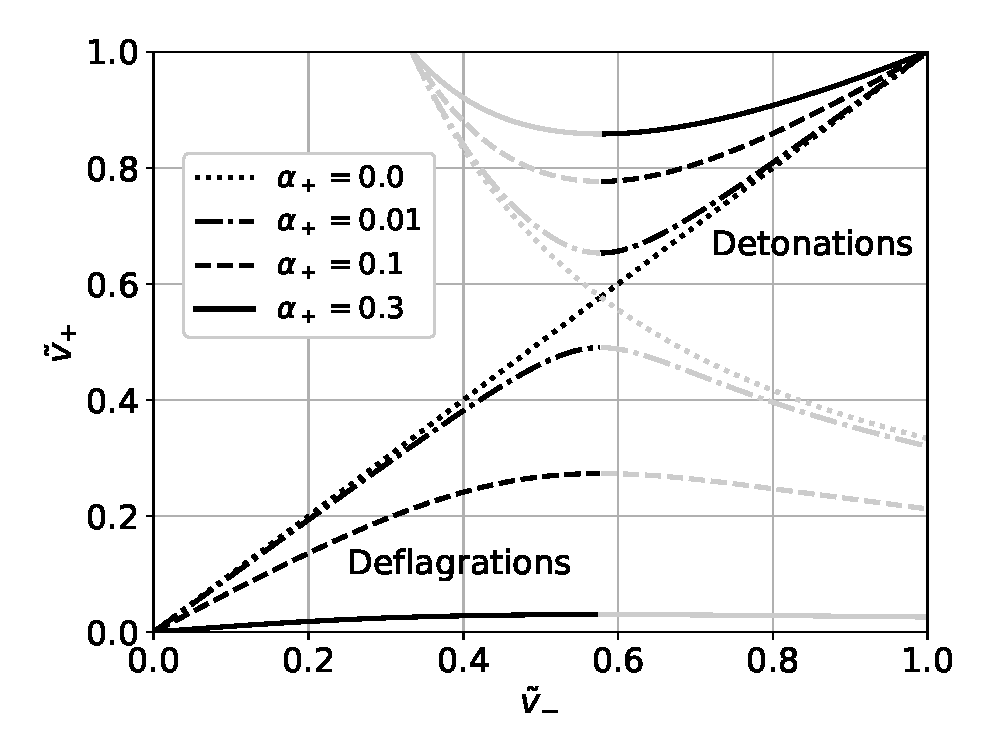
\includegraphics[width=0.7\textwidth]{msc2-python/fig/vm_vp_plane.eps}
\caption{Relation between the fluid velocity just ahead of the wall $\tilde{v}_+$ and just behind the wall $\tilde{v}_-$. Generated with PTtools. See also \cite[fig. 13]{lecture_notes}.}
\label{fig:vplus_vminus}
\end{figure}
\todo{Explain the blue points}

We can obtain useful continuity equations from the conservation of energy-momentum.
We start by defining two vectors, the fluid 4-velocity
\begin{equation}
u^\mu \equiv \gamma(1, \overrightarrow{v})^\mu
\label{eq:u_mu}
\end{equation}
and its orthonormal vector
\begin{equation}
\bar{u}^\mu \equiv \gamma(v, \frac{\overrightarrow{v}}{v})^\mu.
\end{equation}
\todo{Check the signs of the time components.}
Please note that the way these vectors are defined and the convention for the signature of the metric vary
from article to article.
These vectors form an orthonormal basis.
It should be noted, that for orthonormal vectors
% Note that the lecture notes use ubar here.
\begin{align}
u_\mu u^\mu &= 1, \\
u_\mu \bar{u}^\mu &= 0.
\end{align}
\cite[p. 36]{lecture_notes}
By projecting the conservation equation~\eqref{eq:ep_conservation} to this basis and noting that
$\nabla_\nu (u_\mu u^\mu) = 0$ and therefore $u_\mu \nabla_\nu u^\mu = 0$, we get
\cite[eq. 7.28-7.29]{lecture_notes}
\begin{align}
0 &= u_\mu \nabla_\nu T^{\mu \nu} = -\nabla_\mu (w u^\mu) + u^\mu \nabla_\mu p,
\label{eq:continuity1} \\
0 &= \bar{u}_\mu \nabla_\nu T^{\mu \nu} = w \bar{u}^\nu u^\mu \nabla_\mu u_\nu + \bar{u}^\mu \nabla_\mu p.
\label{eq:continuity2}
\end{align}
These are known as the continuity equations, or the hydrodynamic equations.
It should be noted that many articles use the symbol of a partial derivative $\partial$ in these equations,
even though it's actually a covariant derivative $\nabla$.
Since we are operating in spherical coordinates,
the divergence of a vector $A$ is given by
\begin{align}
\nabla \cdot A
% &= \partial_r A^r + \partial_\theta A^\theta + \partial_\phi A^\phi \\
&= \frac{1}{r^2} \frac{\partial (r^2 A^r)}{\partial r}
+ \frac{1}{r \sin \theta} \frac{\partial A^\theta}{\partial \theta}
+ \frac{1}{r \sin \theta} \frac{\partial A^\phi}{\partial \phi}.
\label{eq:divergence}
\end{align}
Let us look for a spherically symmetric self-similar solution using the dimensionless coordinate
\begin{equation}
\xi \equiv \frac{r}{t}.
\label{eq:xi}
\end{equation}
In a spherically symmetric case for $u^\mu$ of eq.~\eqref{eq:u_mu},
the latter two terms of~\eqref{eq:divergence} are zero, and therefore
\begin{equation}
\nabla_\mu u^\mu = \frac{\gamma}{t} \left[ 2\frac{v}{\xi} + \left[1 - \gamma^2 v (\xi - v) \right] \frac{\partial v}{\partial \xi} \right]
\end{equation}
The gradients in~\eqref{eq:continuity1} and~\eqref{eq:continuity2} can also be expressed as~\cite[eq. 25]{espinosa_energy_2010}.
\begin{align}
u_\mu \nabla^\mu &= - \frac{\gamma}{t} (\xi - v) \frac{\partial}{\partial \xi}, \\
\bar{u}_\mu \nabla^\mu &= \frac{\gamma}{t} (1 - \xi v) \frac{\partial}{\partial \xi}.
\end{align}
With these eq.~\eqref{eq:continuity1} and~\eqref{eq:continuity2} can be expressed as
\begin{align}
(\xi - v) \frac{1}{w} \frac{de}{d\xi} &= 2 \frac{v}{\xi} + \left[ 1 - \gamma^2 v (\xi - v) \right] \frac{dv}{d\xi}, \\
(1 - v\xi) \frac{d_\xi p}{w} &= \gamma^2 (\xi - v) \frac{dv}{d\xi}.
\end{align}
These are dependent only on $\xi$ instead of $r$,
and therefore a spherically symmetric self-similar solution exists.
Here the derivatives are now total derivatives, as $e$ and $p$ are functions of a single variable.
By dividing one equation by the other and using eq.~\eqref{eq:cs2_compact}, we can combine these to
\begin{equation}
2 \frac{v}{\xi} = \gamma^2 (1 - v\xi) \left[ \frac{\mu^2}{c_s^2} - 1 \right] \frac{dv}{d\xi},
\label{eq:continuity_combined}
\end{equation}
where
\begin{equation}
\mu(\xi,v) \equiv \frac{\xi - v}{1 - \xi v}
\label{eq:mu}
\end{equation}
is the
Lorentz transformed fluid velocity
$\xi$ in a frame moving outward with the speed $v$.
This can be rearranged to give
\cites[eq. 7.30-7.31]{lecture_notes}[eq. 5]{giese_2021}
\begin{equation}
\frac{dv}{d\xi} = \frac{2v(1-v^2)}{\xi(1-v\xi)} \left( \frac{\mu(\xi,v)^2}{c_s^2} - 1 \right)^{-1}.
\label{eq:hydro_diff1}
\end{equation}
From eq.~\eqref{eq:continuity2} using eq.~\eqref{eq:cs2_compact} and~\eqref{eq:enthalpy_sum} we also get
\begin{equation}
\frac{dw}{d\xi} = w \left( 1 + \frac{1}{c_s^2} \right) \gamma^2 \mu(\xi,v) \frac{dv}{d\xi}.
\label{eq:hydro_diff2}
\end{equation}

Equation~\eqref{eq:hydro_diff1} can be split in two using an auxiliary quantity $\tau$,
resulting in the equation group
\cite[eq. B.14-16]{hindmarsh_gw_pt_2019}
\begin{align}
\frac{d\xi}{d\tau} &= \xi \left[ (\xi - v)^2 - c_s^2 (1 - \xi v)^2 \right],
\label{eq:hydro_param1} \\
\frac{dv}{d\tau} &= 2 v c_s^2 (1 - v^2) (1 - \xi v),
\label{eq:hydro_param2} \\
\frac{dw}{d\tau} &= w \left( 1 + \frac{1}{c_s^2} \right) \gamma^2 \mu \frac{dv}{d\tau}.
\label{eq:hydro_param3}
\end{align}
This is easier to prove in the reverse direction by dividing one equation by the other.
It should be noted that in general $c_s^2 = c_s^2(w,\phi)$, which tightens the coupling between these equations.
The parametric equations have fixed points at
$(\xi,v) = (0,0)$ and
$(\xi,v) = (1,1)$.
When $c_s$ is a constant, the equations also have a fixed point at
$(\xi,v) = (c_s,0)$.
When $c_s$ is constant, the first two equations are not dependent on enthalpy, which simplifies the integration considerably.
However, in the general case of $c_s(w,\phi)$ the equations have to be integrated together.
\todo{Add $(\xi,v)$ plots to the models and refer to them here.}

\section{Types of solutions}
Solutions to the hydrodynamic equations~\eqref{eq:hydro_param1},~\eqref{eq:hydro_param2} are obtained by integrating away from the position of the bubble wall, $\xi_w$.
There are two relevant external boundary conditions.
To maintain spherical symmetry
\begin{equation}
\lim_{\xi \rightarrow 0} v = 0.
\end{equation}
To maintain causality
\begin{equation}
\lim_{\xi \rightarrow 1} v = 0,
\end{equation}
as no information can propagate faster than light, and we assume the fluid to be stationary until a signal from the expanding bubble arrives.
In addition to these there is one boundary condition for each side of the wall as
\begin{equation}
\lim_{\xi \rightarrow \xi_w^\pm = v_w \pm \delta, \delta \rightarrow 0} v = v_\pm = \mu (\xi_w, \tilde{v}_\pm),
\end{equation}

There are two ways to satisfy these conditions.
We can either start at $v=0$, or from a region where $\xi > c_{s-}(w)$ and $\mu(\xi,v) > c_{s-}(w)$, and therefore $\frac{dv}{d\xi} > 0$,
and integrating backwards in $\xi$ over a route where $\mu(\xi,v) > c_{s-}(w)$ is satisfied.
The other way to reach $v=0$ is by a discontinuity, i.e. a shock.
This leads to two classes of solutions.
Another way to see that there are two classes of solutions is by noting
that the equations \eqref{eq:v_tilde_plus} and \eqref{eq:v_tilde_minus} have two branches.
These solutions are classified in table \ref{table:solution_types}.

The solutions with $\tilde{v}_+ > \tilde{v}_-$ are known as detonations.
% In this case there is no way for the front to influence the fluid ahead,
% and the outermost front is a shock.
Detonations are further characterised by the scale of their $\tilde{v}_-$.
In weak detonations $\tilde{v}_- > c_{s-}(w_-)$.
However, weak detonations are not possible in an exothermic reaction such as a cosmological phase transition.
\cite[p. 265]{rezzolla_relativistic_2013}
\todo{According to Hindmarsh weak detonations could exist. Check whether this is possible!}
\todo{How should we modify the $(\xi,v)$ plot for weak detonations to appear?}
Correspondingly, detonations with $\tilde{v}_- < c_{s-}(w_-)$ are known as strong detonations.
However, they are unstable and will naturally evolve into the third class of detonations,
the Chapman-Jouguet detonations, for which $\tilde{v}_- = c_{s-}(w_-)$.
\cite[p. 279]{rezzolla_relativistic_2013}
Since we are investigating a self-similar bubble that has already evolved for some time,
all our detonations of interest are Chapman-Jouguet detonations.
\todo{What would a strong detonation look like in the $(\xi,v)$ plot?}
In Chapman-Jouguet detonations the shock and phase boundary fronts are unified to a single front.

The solutions where $\tilde{v}_+ < \tilde{v}_-$ are known as deflagrations.
In them the phase front can influence the fluid ahead, and the wall is preceded by an accelerating fluid and a shock.
Like with weak detonations, strong deflagrations are not possible in an exothermic reaction.
\cite[p. 267]{rezzolla_relativistic_2013}
Therefore only weak and Chapman-Jouguet deflagrations are possible.
In weak detonations the fluid inside the phase boundary is still, and the preceding shock is weak and
known as the precompression front.

In several articles \cites[p. 37]{lecture_notes}[p. 35]{hindmarsh_gw_pt_2019}
Chapman-Jouguet deflagrations are known as supersonic deflagrations or hybrids,
\todo{Chapman-Jouguet detonations are the fastest, but the relation between hybrids and C-J is not one-to-one. Fix this}
as in them the wall speed exceeds the speed of sound in the broken phase $c_{s-}$,
and the fluid is moving inside the phase boundary as well, as in a detonation.
\todo{Investigate what a strong detonation looks like.}

\begin{table}[ht!]
\small
\begin{tabular}{r|c|c}
                & Detonations            & Deflagrations \\
                & $p_+ < p_-, \tilde{v}_+ > \tilde{v}_-$ & $p_+ > p_-, \tilde{v}_+ < \tilde{v}_-$ \\ \hline
Weak            & {\color{gray} $\tilde{v}_+ > c_{s+}(w_+), \ \tilde{v}_- > c_{s-}(w_-)$} & $\tilde{v}_+ < c_{s+}(w_+), \ \tilde{v}_- < c_{s-}(w_-)$ \\
Chapman-Jouguet & $\tilde{v}_+ > c_{s+}(w_+), \ \tilde{v}_- = c_{s-}(w_-)$ & $\tilde{v}_+ < c_{s+}(w_+), \ \tilde{v}_- = c_{s-}(w_-)$ \\
Strong          & {\color{gray} $\tilde{v}_+ > c_{s+}(w_+), \ \tilde{v}_- < c_{s-}(w_-)$} & {\color{gray} $\tilde{v}_+ < c_{s+}(w_+), \ \tilde{v}_- > c_{s-}(w_-)$} \\
\end{tabular}
\label{table:solution_types}
\end{table}

\begin{figure}[h!]
\centering
\missingfigure{TODO}
\caption{Three different types of relativistic combustion \cite[fig. 14]{lecture_notes}}
\label{fig:solution_types}
\end{figure}


\clearpage
\FloatBarrier
\subsection{Speed limits}
The observables of a physical system must be real, including $\tilde{v}_+$ and $\tilde{v}_-$.
Therefore the expressions in the square roots of \eqref{eq:v_tilde_plus} and \eqref{eq:v_tilde_minus} must be real.
By simplifying the expression in the square root of \eqref{eq:v_tilde_plus} we see that the square root is real $\forall \alpha_+ \geq 0$,
but setting the square root in \eqref{eq:v_tilde_minus} to zero gives a limit for $\tilde{v}_+$ as
\begin{equation}
\tilde{v}_+ = \frac{1}{\sqrt{3}} \left( \frac{1 \pm \sqrt{2 \alpha_+ + 3 \alpha_+^2}}{1 + \alpha_+} \right).
\label{eq:v_tilde_plus_limit}
\end{equation}
The positive sign is the lower limit for detonations, and the negative sign is the upper limit for deflagrations.
\footnote{This is the same equation as in \cites[eq. 7.34]{lecture_notes}[eq. B.19]{hindmarsh_gw_pt_2019},
but in those articles there is a typo due to which a factor of 2 is missing from the expression.}

Inserting this value to the equation \eqref{eq:v_tilde_minus} and simplifying the expression with the knowledge that the square root is now zero
we get that
\begin{equation}
\tilde{v}_- = \frac{1}{\sqrt{3}}.
\label{eq:v_tilde_minus_limit}
\end{equation}
This is the lower limit for detonations, and the upper limit for deflagrations.

The Chapman-Jouguet speed is defined as
\begin{equation}
\tilde{v}_+=v_{CJ} \Leftrightarrow \tilde{v}_- = c_{s-}(w_-).
\label{eq:chapman_jouguet}
\end{equation}
Starting from section \eqref{bag_model} we will see that for some models the speed limit set by the Chapman-Jouguet speed of \eqref{eq:chapman_jouguet}
and the condition of \eqref{eq:v_tilde_minus_limit} that the observables are real are equivalent,
but in general this is not the case.

Now we have the necessary knowledge to classify the different regions of fig. \eqref{fig:vplus_vminus}.
If the speeds of sound are equivalent to $\frac{1}{\sqrt{3}}$,
we can have only weak and Chapman-Jouguet detonations and deflagrations.
However, the weak detonations are ruled out for the aforementioned reason that they are not possible in an exothermic reaction.

When the speed of sound in the broken phase $c_{s-}(w_-) < \frac{1}{\sqrt{3}}$,
we can have a strong deflagration where $c_{s-}(w_-) < \tilde{v}_- < \frac{1}{\sqrt{3}}$.
Correspondingly, when $c_{s-}(w_-) > \frac{1}{\sqrt{3}}$,
we can have a strong detonation where $\frac{1}{\sqrt{3}} < \tilde{v}_-(w_-, \phi_-) < c_{s-}(w_-)$.
However, as previously discussed, a strong detonation is unstable and will evolve into a Chapman-Jouguet detonation.
Since for Chapman-Jouguet detonations $v_w = \tilde{v}_+ > \tilde{v}_-$,
the Chapman-Jouguet speed is the lower speed limit for detonations that have been evolving for a sufficiently long time.


\section{General equation of state}
\label{general_eq}
The equation of state is the function $p(T)$ or $p(w)$ that characterises the behaviour of the fluid as a function of temperature $T$ or enthalpy $w$.
It should be highlighted that everything up to this point has been independent of the equation of state.
We will now first describe the derivation for the general equation of state of an ultrarelativistic plasma,
and then introduce approximate models.

\iffalse
In general the pressure of the ultrarelativistic ASDF
\begin{equation}
p(T,\phi) = - \sum_B f_B (m(\phi),T) - \sum_F f_F (m(\phi),T)
\end{equation}
\fi

The energy density at a point is the sum of the energies of all particles at that point.
Therefore the energy density in the position space can be obtained by integrating over the momentum space as
\cite[eq. 4.10]{lecture_notes}
\begin{equation}
e(x) = \int \frac{d^3 p}{(2 \pi)^3} E(p) f(\vec{p}, x).
\end{equation}
\href{https://physics.stackexchange.com/a/141737/}{The factor $(2\pi)^3$ normalises the momentum space}.
Similarly we can obtain the other components of the energy-momentum tensor in the position space as
\cite[eq. 4.13]{lecture_notes}
\begin{equation}
T^{\mu \nu}(x) = \int \frac{d^3 p}{(2 \pi)^3} \frac{p^\mu p^\nu}{p^0} f(\vec{p},x).
\end{equation}
To give an intuitive explanation for this we can note that $p^0 = E = \gamma m_0$ and $p^i = \gamma m_0 v^i$,
Therefore $\frac{p^i}{p^0} = v^i$,
and the factor $\frac{p^i p^j}{p^0} = p^i v^j$ denotes the amount of momentum being transported by the moving plasma.
By inserting this to the definition of pressure \eqref{eq:pressure_from_ep_tensor} we get
\begin{equation}
p(x) = \frac{1}{3} \int \frac{d^3 p}{(2 \pi)^3} \frac{|\vec{p}|^2}{E} f(\vec{p},x)
\end{equation}
This notation is rather confusing, as the $p$ on the left refers to the pressure,
and all $p$ on the right refer to the momentum.

The particle distribution functions for fermions and bosons are
\cite[eq. 4.6]{lecture_notes}
\begin{equation}
f(\vec{p}) = \frac{1}{e^\frac{E-\mu}{T} \pm 1},
\end{equation}
where $+$ gives the Fermi-Dirac distribution for fermions and $-$ gives the Bose-Einstein distribution for bosons.
Let us approximate that the fluid consists entirely of bosons,
and that they are ultrarelativistic: $E(\vec{p}) = \sqrt{\vec{p}^2 + m^2} \approx p$.
Particle number is not conserved in an ultrarelativistic plasma, and therefore $\mu = 0$.
Let us also remember that we can convert the integral to 1D using the area of a sphere $A(r) = 4\pi r^2$.
With these we get
\begin{align}
e &= \frac{1}{2 \pi^2} \int_0^\infty \frac{p^3 dp}{e^\frac{p}{T} - 1},
\label{eq:ultrarelativistic_e} \\
p &= \frac{1}{6 \pi^2} \int_0^\infty \frac{p^3 dp}{e^\frac{p}{T} - 1}.
\label{eq:ultrarelativistic_p}
\end{align}
These contain integrals of the form
\cite[eq. B.36]{schroeder_thermal_2000}
\begin{equation}
\int_0^\infty \frac{x^n}{e^x - 1} = \Gamma(n+1) \zeta(n+1),
\end{equation}
where $\Gamma$ is the
\href{https://en.wikipedia.org/wiki/Gamma_function}{gamma function}, which for integers is $\Gamma(n) = (n-1)!$.
$\zeta$ is the
\href{https://en.wikipedia.org/wiki/Riemann_zeta_function}{Riemann zeta function}.
It can be shown that $\zeta(4) = \frac{\pi^4}{90}$.
\cite[prob. B.19]{schroeder_thermal_2000}
At this ultrarelativistic limit we can see from eq. \eqref{eq:ultrarelativistic_e} and \eqref{eq:ultrarelativistic_p} that $e = 3p$, and therefore using eq. \eqref{eq:cs2_compact} $c_s^2 = \frac{1}{3}$.

To account for the various particle species in the plasma and their non-ultrarelativistic behaviour,
we need to multiply with the degrees of freedom $g_e$ and $g_p$,
which are weighted sums over the contributions of different particle species.
To also account for the field, we need to add its potential $V$ to the final result
\cite[eq. S12]{borsanyi_lattice_2016}
\begin{align}
e(T,\phi) &= \frac{\pi^2}{30} g_e(T) T^4 + V(T,\phi),
\label{eq:e_general} \\
p(T,\phi) &= \frac{\pi^2}{90} g_p(T) T^4 - V(T,\phi).
\label{eq:p_general}
\end{align}

With \eqref{eq:enthalpy_sum}, \eqref{eq:enthalpy_entropy}, \eqref{eq:e_general} and \eqref{eq:p_general} we can obtain the entropy density as
\cite[eq. S12]{borsanyi_lattice_2016}
\begin{equation}
s(T,\phi) = \frac{2\pi^2}{45} g_s(T) T^3,
\end{equation}
\todo{Should the entropy be defined differently? Defining it with $s = \frac{dp}{dT}$ results in a much more complex and less useful expression.}
where the degrees of freedom for the entropy density are
\begin{equation}
g_s = \frac{1}{4} (3g_e + g_p).
\end{equation}
Often only $g_e$ and $g_s$ are provided, and $g_p$ is obtained with
\begin{equation}
g_p = 4g_s - 3g_e.
\end{equation}
For a free scalar particle $g_e = g_p = g_s = 1$, which is known as the Stefan-Boltzmann limit.
\iffalse
due to its reminiscence to the Stefan-Boltzmann law $j^* = \sigma T^4$,
which relates the power radiated by a black body to its temperature with the Stefan-Boltzmann constant $\sigma$.
\fi

% \clearpage
\section{The bag model}
\label{bag_model}
For phase transitions in the early universe,
the most commonly used equation of state is the bag model, for which
\begin{equation}
g_{e\pm} = g_{p\pm} = g_{s\pm} = \frac{90}{\pi^2} a_\pm,
\end{equation}
where $a_\pm$ are constants with $a_+ > a_-$.
$+$ refers to the symmetric phase, and $-$ refers to the broken phase.
The potentials $V_\pm$ are also constants with $V_+ > V_-$.
This results in the bag equation of state
\cites[eq. 7.33]{lecture_notes}[eq. 8-9]{giese_2020}
\begin{equation}
p_\pm = a_\pm T^4 - V_\pm.
\label{eq:bag_p}
\end{equation}
The potential difference $\Delta V \equiv V_+ - V_-$, also known as $\epsilon$,
is the temperature-independent vacuum energy that is released in the phase transition.
The potentials are usually shifted so that $V_b = 0$.
The name of the bag model originates from quantum chromodynamics (QCD),
where it's used to describe the proton as a bag of quarks.
\cite{giese_2020}

Using eq.~\eqref{eq:entropy_density} we get the entropy density
\begin{equation}
s_\pm = 4 a_\pm T^3,
\end{equation}
and with eq.~\eqref{eq:enthalpy_entropy} the enthalpy density
\begin{equation}
w_\pm = 4 a_\pm T^4.
\end{equation}
Finally with eq.~\eqref{eq:enthalpy_sum} we get the energy density
\begin{equation}
e_\pm = 3 a_\pm T^4 + V_\pm.
\end{equation}
The speed of sound from eq.~\eqref{eq:cs2_explicit} simplifies to
\begin{equation}
c_s^2 = \frac{dp}{de} = \frac{dp/dT}{de/dT} = \frac{1}{3}.
\end{equation}
As in section~\ref{general_eq}, this corresponds to assuming both of the phases to be ultrarelativistic.
It also happens to be the same as the $\tilde{v}_-$ that corresponds to eq.~\eqref{eq:v_tilde_plus_limit},
and therefore the Chapman-Jouguet speed $v_{CJ}$ of the bag model is given by eq.~\eqref{eq:v_tilde_plus_limit}.
The trace anomaly of eq.~\eqref{eq:theta} simplifies to
\begin{align}
\theta_\pm = V_\pm.
\end{align}
Therefore, the transition strength of~\eqref{eq:alpha_plus} simplifies to
\begin{equation}
\alpha_{+,\text{bag}} = \frac{4 \Delta V}{3 w_+},
\label{eq:alpha_plus_bag}
\end{equation}
and the transition strength at nucleation temperature from~\eqref{eq:alpha_n} simplifies to
\begin{equation}
\alpha_{n,\text{bag}} = \frac{4 \Delta V}{3 w_n}.
\label{eq:alpha_n_bag}
\end{equation}
This is trivial to invert, giving enthalpy at the nucleation temperature $w_n$.

% \clearpage
\section{More complex models}
The bag model is a rather crude approximation, and for realistic simulations a more complex model is needed.
In general, the model for an equation of state is constructed by providing two of $g_e, g_p$ and $g_s$,
or equivalently two of $e, p$ and $s$, and the potential $V(T,\phi)$.
The rest of the model properties can be computed from these.

\iffalse
\begin{itemize}
    \item Bubble wall velocity $v_w$
    \item Nucleation temperature $T_n$, or equivalently nucleation enthalpy $w_n$ or transition strength $\alpha_n$
    \item Phase transition duration $\frac{1}{\beta}$ \todo{Check this}
    \item Equation of state
    \item Fraction of energy that is converted into fluid motion: $\kappa$ (???)
    \item Numerical prefactor from lattice simulations (???)
\end{itemize}
\fi


\subsection{The constant sound speed model}
\label{const_cs}
The constant sound speed model, also known as the $\mu_\pm$ model, the $\mu, \nu$ model,
or in some sources as the template model,
expands the bag model by allowing a different speed of sound in each phase.
It is obtained by setting
\begin{equation}
g_{p\pm} = \frac{90}{\pi^2} a_\pm \left( \frac{T}{T_0} \right)^{\mu_\pm - 4},
\end{equation}
where $\mu_\pm$ are constants.
This results in the equation of state
\cites[eq. 15]{giese_2021}[eq. 38]{giese_2020}
\begin{equation}
p_\pm = a_\pm \left( \frac{T}{T_0} \right)^{\mu_\pm - 4} T^4 - V_\pm {\color{gray} \approx a_\pm T^{\mu_\pm} - V_\pm }, \\
\end{equation}
The reference temperature $T_0$ is introduced for the consistency of the units.
For simplicity it can be set to 1 GeV, or whichever unit one is using for the temperature.
The greyed-out version is commonly seen in articles and useful, but has inconsistent units.
The parameters $\mu_\pm$ are determined by the sound speeds in the symmetric and broken phases with
\cites[eq. 16]{giese_2021}[eq. 39]{giese_2020}
\footnote{Please note that there is a typo in \cite[eq. 15]{giese_2021}. There the 4 should be a $\mu$.}
\begin{equation}
\mu_\pm \equiv 1 + \frac{1}{c_{s\pm}^2},
\end{equation}
This model reduces to the bag model,
when $c_{s+}^2 = c_{s-}^2 = \frac{1}{3}$
and equivalently
$\mu_+ = \mu_- = 4$.

Similarly as for the bag model we can derive the entropy density
\begin{equation}
s_\pm = \mu_\pm a_\pm \left( \frac{T}{T_0} \right)^{\mu_\pm - 4} T^3,
\end{equation}
and from it the enthalpy density
\begin{equation}
w_\pm = \mu_\pm a_\pm \left( \frac{T}{T_0} \right)^{\mu_\pm - 4} T^4
\label{eq:w_const_cs}
\end{equation}
and finally the energy density
\begin{equation}
e_\pm = (\mu_\pm - 1) a_\pm \left( \frac{T}{T_0} \right)^{\mu_\pm - 4} T^4 + V_\pm.
\end{equation}
The equation for enthalpy density \eqref{eq:w_const_cs} can be inverted to give the temperature as a function of enthalpy
\begin{equation}
T_\pm = \left( \frac{w}{\mu_\pm a_\pm T_0^4} \right)^\frac{1}{\mu_\pm} T_0,
\end{equation}
Therefore the effective degrees of freedom are
\begin{align}
g_{p\pm} &= \frac{90}{\pi^2} a_\pm \left( \frac{T}{T_0} \right)^{\mu_\pm - 4}, \\
g_{s\pm} &= \frac{45}{2\pi^2} \mu_\pm a_\pm \left( \frac{T}{T_0} \right)^{\mu_\pm - 4}, \\
g_{e\pm} &= \frac{30}{\pi^2} (\mu - 1) a_\pm \left( \frac{T}{T_0} \right)^{\mu_\pm - 4}.
\end{align}


The trace anomaly of \eqref{eq:theta} simplifies to
\begin{align}
\theta_\pm(w)
&= \left( \frac{\mu_\pm}{4} - 1 \right) a_\pm \left( \frac{T}{T_0} \right)^{\mu_\pm - 4} T^4 + V_\pm \\
&= \left( \frac{1}{4} - \frac{1}{\mu_\pm} \right) w_\pm + V_\pm
\label{eq:theta_const_cs}
\end{align}
The transition strength of \eqref{eq:alpha_plus} simplifies to
\begin{equation}
\alpha_+ = \frac{1}{3} \left( 1 - \frac{4}{\mu_+} \right) - \frac{1}{3} \left(1 - \frac{4}{\mu_-} \right) \frac{w_-}{w_+} + \alpha_{+,\text{bag}}.
\label{eq:alpha_plus_const_cs}
\end{equation}
The transition strength at nucleation temperature of \eqref{eq:alpha_n} is correspondingly
\begin{align}
\alpha_n &= \frac{1}{3} \left( 1 - \frac{4}{\mu_+} \right) - \frac{1}{3} \left(1 - \frac{4}{\mu_-} \right) \frac{w(T_n, \phi_-)}{w_n} + \alpha_{n,\text{bag}} \\
&= \frac{4}{3} \left( \frac{1}{\mu_-} - \frac{1}{\mu_+} \right) + \frac{1}{3} \left( 1 - \frac{4}{\mu_-} \right)
\left( 1 - \frac{\mu_- a_-}{\mu_+ a_+} \left( \frac{T_n}{T_0} \right)^{\mu_- - \mu_+} \right) + \alpha_{n,\text{bag}}
\label{eq:alpha_n_const_cs}
\end{align}
\iffalse
% This is wrong
Inverting this gives the enthalpy at the nucleation temperature
\begin{equation}
w_n = \frac{V_+ - V_-}{ \frac{3}{4} \alpha_n + \frac{1}{\mu_+} - \frac{1}{\mu_-} }.
\label{eq:wn_const_cs}
\end{equation}
\fi
When $\mu_- = 4$, $\alpha_n$ of \eqref{eq:alpha_n_const_cs} becomes independent of $w_-$, resulting in
\begin{equation}
w_n = \frac{4 (V_+ - V_-)}{3 \alpha_n + \frac{4}{\mu_+} - 1}.
\label{eq:wn_const_cs_mu4}
\end{equation}
In this case we can obtain $v_{CJ}(\alpha_n, c_{s+})$ analytically.
First we insert $\alpha_n$ to \eqref{eq:wn_const_cs_mu4} to get $w_n$,
and then insert $w_n$ to \eqref{eq:alpha_plus_const_cs} to get $\alpha_+$,
since in this case $\alpha_+$ is independent of $w_-$.
Then we can insert $c_{s-}$ and $\alpha_+$ to \eqref{eq:v_tilde_plus} to get $\tilde{v}_+ = v_{CJ}$.

\iffalse
Now we have everything necessary to compute $\alpha_+$ and the Chapman-Jouguet speed $v_{CJ}$ analytically from $c_{s+}$, $c_{s-}$ and $\alpha_n$.
From these we get $w_n$ with \eqref{eq:wn_const_cs}, and for a detonation $w_+=w_n$.
This we can insert to \eqref{eq:wm_const_cs}, giving us $w_-$.
Now we have all the variables necessary to compute $\alpha_+$ with \eqref{eq:alpha_plus}.
Then we insert $\tilde{v}_- = c_{s-}$ to \eqref{eq:v_tilde_plus}, giving us the Chapman-Jouguet speed $v_{CJ} = v_+$.
\todo{This is wrong! We have a circular dependency and must solve the equation group at once.}
\fi

The pseudotrace of \eqref{eq:theta_bar} is given by
\begin{align}
\bar{\theta} = (\mu_\pm - \mu_-) a \left(\frac{T}{T_0}\right)^{\mu_\pm - 4} T_0^4 + \mu_- V_\pm.
\end{align}
Therefore the corresponding transition strengths of \eqref{eq:alpha_theta_bar_plus} and \eqref{eq:alpha_theta_bar_n} become
\begin{align}
\alpha_{\bar{\theta}_+} &= \frac{1}{3} \left(1 - \frac{\mu_-}{\mu_+}\right) + \frac{\mu_-}{4} \alpha_{+,\text{bag}}, \\
\alpha_{\bar{\theta}_n} &= \frac{1}{3} \left(1 - \frac{\mu_-}{\mu_+}\right) + \frac{\mu_-}{4} \alpha_{n,\text{bag}}.
\end{align}
These are equal for detonations regardless of the wall speed or the speeds of sound,
since $\alpha_{+,\text{bag}} = \alpha_{n,\text{bag}}$ for detonations.

If we set $T_0 = T_c$, eq. \eqref{eq:critical_temp} results in
\begin{equation}
\Delta V = (a_+ - a_-) T_c^4.
\end{equation}
Using this the "bag" part in eq. \eqref{eq:alpha_plus_const_cs} and \eqref{eq:alpha_n_const_cs} becomes
\begin{align}
\alpha_{+,\text{bag}} &= \frac{4}{3 \mu_+} \left( 1 - \frac{a_-}{a_+} \right) \left( \frac{T_+}{T_c} \right)^{-\mu_+}, \\
\alpha_{n,\text{bag}} &= \frac{4}{3 \mu_+} \left( 1 - \frac{a_-}{a_+} \right) \left( \frac{T_n}{T_c} \right)^{-\mu_+}.
\end{align}
Using this we can reorder \eqref{eq:alpha_n_const_cs} to
\begin{equation}
\frac{a_-}{a_+} = \frac{4 + \left( \mu_+ - 4 - 3 \mu_+ \alpha_n \right) \left(\frac{T_n}{T_c}\right)^{\mu_+}}{4 + \left( \mu_- - 4 \right) \left(\frac{T_n}{T_c}\right)^{\mu_-}}.
\end{equation}
Noting that $T_n < T_c$, this restricts $\alpha_n$ to
\begin{equation}
\alpha_n > \frac{\mu_+ - \mu_-}{3 \mu_+}.
\end{equation}
Even though we have used $T_0 = T_c$ in the intermediate steps, this restriction is general.

Approximating $T_+ \approx T_-$ results in eq. \eqref{eq:cs2_compact} being approximated as
\begin{equation}
c_{s,b}^2
\equiv \frac{dp_b}{de_b}
= \frac{dp_b/dT}{de_b/dT} \big|_{T_+ \approx T_-}
\approx \frac{\delta p_-}{\delta e_-}.
\label{eq:const_cs_approx}
\end{equation}
In the case of the constant sound speed model $c_{s}$ is independent of temperature, and therefore this approximation is exact.
With this approximation and the use of eq. \eqref{eq:delta_relation} the second junction condition of eq. \eqref{eq:junction_conditions_simplified} becomes
\begin{equation}
\delta p_- \left(1 - \frac{\tilde{v}_+ \tilde{v}_-}{c_{s,b}^2} \right) = \tilde{v}_+ \tilde{v}_- De_+ - Dp_+
\end{equation}
Using this, eq. \eqref{eq:delta_relation} and eq. \eqref{eq:enthalpy_sum} on the first junction condition of \eqref{eq:junction_conditions_simplified} results in
\begin{align}
\frac{\tilde{v}_+}{\tilde{v}_-}
&\approx \frac{
w_+ \left( \frac{\tilde{v}_+ \tilde{v}_-}{c_{s,b}^2} - 1 \right) + \left( De_+ - \frac{Dp_+}{c_{s,b}^2} \right)
}{
w_+ \left( \frac{\tilde{v}_+ \tilde{v}_-}{c_{s,b}^2} - 1 \right) + \tilde{v}_+ \tilde{v}_- \left( De_+ - \frac{Dp_+}{c_{s,b}^2} \right)
} \\
&= \frac{ \left( \frac{\tilde{v}_+ \tilde{v}_-}{c_{s,b}^2} - 1 \right) + 3 \alpha_{\bar{\theta}_+}
}{
\left( \frac{\tilde{v}_+ \tilde{v}_-}{c_{s,b}^2} - 1 \right) + 3\tilde{v}_+ \tilde{v}_- \alpha_{\bar{\theta}_+}}
\label{eq:const_cs_vp_vm}
\end{align}
The only approximation in this calculation is that of eq. \eqref{eq:const_cs_approx}.
As it is exact for the constant sound speed model,
eq. \eqref{eq:const_cs_vp_vm} is exact for the constant sound speed model.
Eq. \eqref{eq:const_cs_vp_vm} can be rearranged to
\begin{equation}
\frac{\tilde{v}_+}{c_{s,b}^2} \tilde{v}_-^2
+ \left(3 \alpha_{\bar{\theta}_+} - 1 - \tilde{v}_+^2 \left(\frac{1}{c_{s,b}^2} + 3 \alpha_{\bar{\theta}_+} \right) \right) \tilde{v}_-
+ \tilde{v}_+
= 0,
\end{equation}
which is a basic second-order equation for $\tilde{v}_- ( \tilde{v}_+, \alpha_{\bar{\theta}_+} )$.
Since $\tilde{v}_+ = v_w$ for all detonations, and $\alpha_{\bar{\theta}_+} = \alpha_{\bar{\theta}_n}$ for all detonations in the constant sound speed model, this gives $\tilde{v}_- ( v_w, \alpha_{\bar{\theta}_n} )$.
And since \eqref{eq:alpha_n_const_cs} gives $\alpha_n(\mu_+, \mu_-, \alpha_{n,\text{bag}}$, we have $\tilde{v}_- (v_w,
$
TODO
Eq. \eqref{eq:const_cs_vp_vm} can also be rearranged to
\begin{equation}
\left( \frac{1}{c_{s,b}^2} + 3\alpha_{\bar{\theta}_+} \right) \tilde{v}_+^2
- \left( \frac{1}{\tilde{v}_-} + \frac{\tilde{v}_-}{c_{s,b}^2} \right) \tilde{v}_+
+ 1 - 3\alpha_{\bar{\theta}_+}
= 0.
\end{equation}
This gives the Chapman-Jouguet speed $\tilde{v}_+ \left( \tilde{v}_- = c_{s,b} \right)$ as
\cite[eq. 55]{giese_2020}
\begin{equation}
v_{CJ} = \frac{ 1 + \sqrt{ 3\alpha_{\bar{\theta}_+} ( 1 - c_{s,b}^2 + 3 c_{s,b}^2 \alpha_{\bar{\theta}_+} ) }}{ \frac{1}{c_{s,b}} + 3 c_{s,b} \alpha_{\bar{\theta}_+}}.
\end{equation}
This holds for all values of $\mu_+$ and $\mu_-$.

% \subsection{Model with cubic thermal effects}
Free energy
\todo{Where does this come from? How to extract the thermal effects?}
\cite[eq. 45]{giese_2020}
\begin{align}
\begin{split}
\textsc{F}(\phi, T) =
&- \frac{a_+}{3} T^4 \\
&+ \lambda \left( \phi^4 - 2E\phi^3 T + \phi^2 \left( E^2 T_\text{cr}^2 + c \left( T^2 - T_\text{cr}^2 \right) \right) \right) \\
&+ \frac{\lambda}{4} \left( c - E^2 \right)^2 T_\text{cr}^4
\end{split}
\end{align}

The minimum of the field potential is given by
\cite[eq. 46]{giese_2020}
\begin{equation}
\phi_\text{min} = \frac{3}{4} ET + \sqrt{\frac{T^2}{2}(\frac{9}{8}E^2 - c) - \frac{T_\text{cr}^2}{2} (E^2 - c)}
\end{equation}


\subsection{Model with a two-step phase transition}
Two scalar fields and two symmetry breakings. Examples: electroweak symmetry, $\mathbb{Z}_2$ symmetry.
Cubic term is neglected.
Pressures are of the form
\cite[eq. 47-48]{giese_2020}
\begin{align}
p_s(T) = \frac{1}{3}a_+ T^4 + (b_+ - c_+ T^2)^2 - b_-^2 \\
p_b(T) = \frac{1}{3}a_+ T^4 + (b_- - c_-T^2)^2 - b_-^2
\end{align}
Compare these to the \eqref{eq:bag_ps}, \eqref{eq:bag_pb}.


\subsection{Standard Model}
In the Standard Model the electroweak phase transition is not of first order but a crossover,
and therefore there is no bubble nucleation.
However, it serves as an important baseline.
The $g_e$ and $g_s$ data for the Standard Model is given by \cite{borsanyi_lattice_2016}.


\clearpage
\section{Energy redistribution}
\label{energy_redistribution}
Once the velocity profile of a bubble is known, it can be used to compute various thermodynamic quantities.

We have assumed that the background spacetime is Minkowski, and that the spacetime does not expand significantly during the phase transition.
Therefore, the total energy of the system is conserved and
\begin{equation}
E = 4 \pi \int_0^R dr r^2 T^{00}
\end{equation}
is a constant for $R$ larger than the fluid velocity profile.
It should be noted that this energy conservation applies only to the total energy system,
and not the energy of the fluid, as there is energy transfer from the field to the fluid.
\cite[p. 21]{lecture_notes}
Correspondingly the mean energy density $\bar{e}$ is defined as \cite[p. 39]{lecture_notes}
\begin{equation}
\bar{e} = \frac{3}{\xi_\text{max}^3} \int_0^{\xi_\text{max}} d\xi \xi^2 e = e(w_n, \phi_s).
\label{eq:e_conservation}
\end{equation}
The mean enthalpy density $\bar{w}$ is defined as
\begin{equation}
\bar{w} = \frac{3}{\xi_\text{max}^3} \int_0^{\xi_\text{max}} d\xi \xi^2 w
\label{eq:wbar}
\end{equation}
Using these we can define the energy fluctuation variable
\begin{equation}
\lambda(x) = \frac{e(x) - \bar{e}}{\bar{w}}.
\label{eq:lambda}
\end{equation}

For an ideal fluid of eq. \eqref{eq:ep_tensor} \cite[eq. B.23]{hindmarsh_gw_pt_2019}
% This is easy to prove by hand.
\begin{equation}
T^{00} = w\gamma^2 - p = w\gamma^2 v^2 + e = w\gamma^2 v^2 + \frac{3}{4}w + \theta.
\end{equation}
Inserting this to the energy conservation equation \eqref{eq:e_conservation} results in the equation \cite[eq. B.24]{hindmarsh_gw_pt_2019}
\begin{equation}
e_K + \Delta e_Q = - \Delta e_\theta,
\label{eq:energy_components}
\end{equation}
which consists of the terms defined below.
The kinetic energy density is given by
\begin{equation}
e_K \equiv 4 \pi \int_0^{\xi_\text{max}} d\xi \xi^2 w \gamma^2 v^2.
\label{eq:kinetic_energy_density}
\end{equation}
It denotes the energy that is converted to macroscopic fluid movement.
The thermal energy density difference is given by
\begin{equation}
\Delta e_Q \equiv 4 \pi \int_0^{\xi_\text{max}} d\xi \xi^2 \frac{3}{4} (w - w_n).
\label{eq:thermal_energy_density}
\end{equation}
It denotes the energy that is converted to microscopic fluid movement.
The trace anomaly difference is given by
\begin{equation}
\Delta e_\theta \equiv 4 \pi \int_0^{\xi_\text{max}} d\xi \xi^2 (\theta - \theta_n).
\end{equation}
It can be considered as the potential energy available for transformation.
We can obtain the volume-average entropy density difference similarly as the energy density, with
\begin{equation}
\Delta s_\text{avg} = 4\pi \int_0^{\xi_\text{max}} d\xi \xi^2 \left( s(w,\phi) - s(w_n, \phi_s) \right).
\end{equation}
The upper integration limit $\xi_\text{max}$ can be chosen arbitrarily as long as it's outside the bubble, as outside the bubble all three quantities go to zero outside the fluid shell due to $v=0$, $w=w_n$ and $\theta = \theta_n$.
A convenient choice is $\xi_\text{max} = \max (v_w, \xi_{sh})$.
\cite[eq. B.25]{hindmarsh_gw_pt_2019}

It should be noted that the trace anomaly is not quite equivalent to the thermal potential energy density $V_T(T,\phi)$, as using eq. \eqref{eq:enthalpy_pressure}, \eqref{eq:enthalpy_sum} and \eqref{eq:p_general} we can see that for the case of temperature-independent $g$,
\begin{equation}
\theta = V_T - \frac{1}{4} T \frac{\partial V_T}{\partial T}.
\end{equation}
Therefore, not all of the potential energy difference can be turned into kinetic and thermal energy.
\cite[ch. B.2]{hindmarsh_gw_pt_2019}

The fraction of total energy that is converted to kinetic energy is known as the kinetic energy fraction,
\begin{equation}
K \equiv \frac{e_K}{\bar{e}}.
\label{eq:kinetic_energy_fraction}
\end{equation}

Kinetic and thermal efficiency factors quantify the fraction of the available energy $\Delta e_\theta$ that is converted to kinetic and thermal energy.
They can be defined as
\begin{equation}
\kappa \equiv \frac{e_K}{| \Delta e_\theta |}, \quad
\omega \equiv \frac{\Delta e_Q}{\Delta e_\theta}.
\label{eq:kappa_omega}
\end{equation}
Since energy is conserved by eq. \eqref{eq:energy_components},
these have have the property that $\kappa + \omega = 1$.

It should be noted that some sources such as \cites[eq. 36]{giese_2020}[eq. 12, 14]{giese_2021}
use different definitions for $\kappa$:
\begin{align}
\kappa_{\bar{\Theta}_+} &\equiv \frac{4 e_K}{D \bar{\Theta}(T_+)} = \frac{4 e_K}{3 \alpha_{\bar{\Theta}_+} w_+},
\label{eq:kappa_thetabar_plus} \\
\kappa_{\bar{\Theta}_n} &\equiv \frac{4 e_K}{D \bar{\Theta}(T_n)} = \frac{4 e_K}{3 \alpha_{\bar{\Theta}_n} w_n}.
\label{eq:kappa_thetabar_n}
\end{align}

The enthalpy-weighted mean square fluid 4-velocity around the bubble is defined by
\begin{equation}
\bar{U}_f^2 = \frac{\Delta e_Q}{w_n}.
\label{eq:ubarf2}
\end{equation}
The adiabatic index is defined as
\begin{equation}
\gamma \equiv \frac{c_P}{c_V},
\end{equation}
where $c_P$ is the specific heat capacity at constant pressure,
and $c_V$ is the specific heat capacity at constant volume.
For a classical monoatomic fluid $\gamma = \frac{5}{3}$,
and for an ultrarelativistic fluid $\gamma = \frac{4}{3}$.
The enthalpy-weighted mean square fluid 4-velocity around the bubble and the kinetic energy density fraction of eq. \eqref{eq:kinetic_energy_fraction} are linked by
\begin{equation}
K = \Gamma \bar{U}_f^2,
\label{eq:kinetic_energy_fraction2}
\end{equation}
where
\begin{equation}
\Gamma \equiv \frac{\bar{w}}{\bar{e}}.
\label{eq:mean_adiabatic_index}
\end{equation}
In the case of the ultrarelativistic bag model $\Gamma$ is the mean adiabatic index,
but for a more general model this may not be the case.


\chapter{Gravitational waves}
\label{ch:gw}
In this thesis the gravitational wave spectrum from the first order phase transition is calculated using the Sound Shell Model.
The Sound Shell Model is the process that converts the fluid velocity and enthalpy profiles of chapter \ref{ch:pt} to the gravitational wave spectra.
This process involves multiple steps.
First in section \ref{gw_production} we investigate how the gravitational wave spectrum is produced by the shear stress.
Then in section \ref{shear_stress} we investigate how the shear stress is produced by the sound waves.
We combine these results in section \ref{gw_from_sound_waves} to see how the gravitational wave spectrum is produced by sound waves.
Then in section \ref{velocity_field} we convert the sound waves the fluid velocity profiles of chapter \ref{ch:pt}.
Combining these, we have the gravitational wave spectra.
These four sections follow the contents and structure in the article \cite{hindmarsh_gw_pt_2019} that introduces the Sound Shell Model.
In section \ref{correction_factors} we extend the process beyond the base Sound Shell Model of the previous sections.
Then in section \ref{omgw0} we convert the results to the frequencies today.
Finally in section \ref{noise} we define the LISA instrument noise to compare the signal-to-noise ratios of the gravitational wave spectra to the LISA instrument noise.


\section{Gravitational wave production from shear stress}
\label{gw_production}
In this section we derive how the gravitational wave spectrum $\mathcal{P}_\text{gw}$ is produced by the shear stress correlator $U_\pi$.
First of all we assume that the time scale of the phase transition is much shorter than the Hubble time.
Therefore we can neglect the expansion of the universe and assume that the background is Minkowski spacetime.
The fluid and the scalar field are sources of metric perturbations for the spacetime.
In the synchronous gauge these produce a change in the space-time interval
\cite[p. 7]{hindmarsh_gw_pt_2019}
\begin{equation}
ds^2 = -dt^2 + (\delta_{ij} + h_{ij}) dx^i dx^j.
\end{equation}
The metric perturbations $h_{ij}$ are sourced by shear stress,
which is the transverse-traceless part of the energy-momentum tensor $\Pi_{ij}$ of eq. \eqref{eq:ep_tensor_general_matrix}.
This results in a wave equation for $h_{ij}$ with a source term,
\cites[eq. 3.1]{hindmarsh_gw_pt_2019}[eq. 1.24]{maggiore_gw_2008}
% (similar to \eqref{eq:wave_equation})
\begin{equation}
\ddot{h}_{ij} - \nabla^2 h_{ij} = 16 \pi G \Pi_{ij}.
\end{equation}
The energy-momentum tensor $T_{ij}$ consists of contributions from the fluid and the scalar field \cite[p. 7]{hindmarsh_gw_pt_2019}
\begin{align}
T^f_{ij}    &= (e+p) \gamma^2 v_i v_j + p \delta_{ij}, \\
T^\phi_{ij} &= \delta_i \phi \delta_j \phi - \frac{1}{2}(\delta \phi)^2 \delta_{ij}.
\end{align}

% Defining P and Lambda tensors
Let us introduce the tensor
\cite[eq. 1.35]{maggiore_gw_2008}
\begin{equation}
P_{ij}(\bm{k}) = \delta_{ij} - \hat{k}_i \hat{k}_j.
\end{equation}
This tensor is symmetric, transverse ($\hat{k}_i P_{ij}(\bm{k}) = 0$) and a projector ($P_{ik}P_{kj} = P_{ij}$), and its trace $P_{ii} = 2$.
Using $P_{ij}$ we can construct another tensor that we call the $\Lambda$ tensor
\cite[eq. 1.36]{maggiore_gw_2008}
\begin{equation}
\Lambda_{ij,kl}(\bm{k}) = P_{ik}(\bm{k}) P_{jl}(\bm{k}) - \frac{1}{2} P_{ij}(\bm{k}) P_{kl}(\bm{k}).
\label{eq:Lambda}
\end{equation}
\iffalse
This is still a projector, in the sense that
\begin{equation}
\Lambda_{ij,kl} \Lambda_{kl,mn} = \Lambda_{ij,mn}.
\end{equation}
It is also transverse on all of its indices as $n^i \Lambda_{ij,kl} = 0$ for all indices ($ijkl$}.
It is traceless with respect to the ($i,j$) and ($k,l$) index pairs,
\begin{equation}
\Lambda_{ii,kl} = \Lambda_{ij,kk} = 0.
\end{equation}
\fi
For further details on the $\Lambda$ tensor, please see
\cite[ch. 1.2]{maggiore_gw_2008}.

% Defining P_\dot{h}
The spectral density of the time derivative of the perturbations, $P_{\dot{h}}(\bm{k},t)$, is defined by
\cite[eq. 3.4]{hindmarsh_gw_pt_2019}%
\footnote{In \cite[eq. 3.4]{hindmarsh_gw_pt_2019} the second $\mathbf{k}$ is a typo and should be $\mathbf{k}'$.}
\begin{equation}
\langle \dot{h}_{\bm{k}}^{ij}(t) \dot{h}_{\bm{k}'}^{ij}(t) \rangle = P_{\dot{h}}(\bm{k},t) (2\pi)^3 \delta (\bm{k} + \bm{k}').
\label{eq:hbracket}
\end{equation}

% Defining e_{gw}, e_c and Omega_gw
The energy density of gravitational waves is given by
\cites[eq. 3.3]{hindmarsh_gw_pt_2019}[eq. 1.135, 7.193]{maggiore_gw_2008}
\begin{align}
e_{gw}
&= \frac{1}{32 \pi G} \int dk^3 \langle \dot{h}_{ij} \dot{h}_{ij} \rangle \\
&= \frac{1}{32 \pi G} \int dk \frac{k^2}{2 \pi^2} P_{\dot{h}}(k).
\end{align}
In many textbooks and articles the integral in the first expression is implicit.
The factor of $\frac{k^2}{2\pi^2}$ results from the conversion to spherical coordinates.
The critical energy density corresponding to a flat universe is given by
\cite[eq. 7.196]{maggiore_gw_2008}
\begin{equation}
e_c = \frac{3 H^2}{8 \pi G}.
\label{eq:e_crit}
\end{equation}
Let us define energy density of gravitational waves relative to the critical energy density.
This is the dimensionless quantity
\begin{equation}
\Omega_{gw} \equiv \frac{e_{gw}}{e_c}.
\label{eq:omega_gw}
\end{equation}
% This will be needed later in eq. \eqref{eq:gw_pow_spec}.

% GW power spectrum. Uses Omega, so this is in the correct place.
The gravitational wave power spectrum is defined by
\cite[eq. 3.45]{hindmarsh_gw_pt_2019}
\begin{equation}
\mathcal{P}_{gw}(k)
\equiv \frac{d \Omega_{gw}}{d \ln (k)}
% = \frac{1}{\bar{\rho}} \frac{1}{32 \pi G} \mathcal{P}_{\dot{h}}(k)
= \frac{1}{12 H^2} \frac{k^3}{2\pi} P_{\dot{h}}(k)
= \frac{1}{12 H^2} \mathcal{P}_{\dot{h}}(k),
\label{eq:gw_pow_spec}
\end{equation}
where the first step is a direct result from the equations above.
It should be noted that in \cite[eq. 3.6, eq. 3.46]{hindmarsh_gw_pt_2019} it is presumed that $\bar{\rho}=e_c$.
A spectral density can be converted to a power spectrum with
\cite[eq. 4.18]{hindmarsh_gw_pt_2019}
\begin{equation}
\mathcal{P}(k) = \textcolor{gray}{(2)} \frac{k^3}{2 \pi^2} P(k).
\label{eq:pow_spec}
\end{equation}
The factor of two is due to the fact that the velocity Fourier transform includes waves moving in both directions.%
\footnote{See also \cite[p. 338]{maggiore_gw_2008}.}
Whether it is included or not is dependent on the context.
Therefore, the gravitational wave power spectrum can be obtained from the spectral density $P_{\dot{h}}$ as
\begin{equation}
\mathcal{P}_{gw}(k) = \frac{1}{12 H^2} \frac{k^3}{2\pi^2} P_{\dot{h}}.
\label{eq:gw_pow_spec2}
\end{equation}
To obtain the gravitational wave spectrum $\mathcal{P}_{gw}(k)$,
we therefore need to obtain an expression for $P_{\dot{h}}$ that we can compute from the fluid shell profile.
For this we will need quite a few similar intermediate quantities.
To avoid confusion, their symbols and names are listed in table \ref{table:symbols}.

% This is here, since the first P has just been introduced.
\begin{table}[ht]
\caption{Symbols and explanations of the spectral quantities}
\begin{tabular}{l|l|l}
Symbol & Explanation & Eq.\\
\hline
$P_{\dot{h}}$ & Spectral density of $\dot{h}$ & \eqref{eq:p_dot_h} \\
$P_v$ & Spec. den. of the plane wave components of the velocity field & \eqref{eq:spec_den_v} \\
% $P_{\tilde{v}}$ & Spec. den. of the Fourier transformation of the velocity field & \eqref{eq:p_tilde_v} \\
$\tilde{P}_v$ & Scaled velocity spectral density & \eqref{eq:tilde_p_v} \\
$\mathcal{P}_{\tilde{v}}$ & Velocity power spectrum & \eqref{eq:pow_v} \\
$\tilde{P}_\text{gw}$ & Spectral density of the gravitational wave power spectrum & \eqref{eq:spectral_density} \\
% $\mathcal{P}_v$ & ??? \\
$\mathcal{P}_\text{gw}$ & Gravitational wave power spectrum & \eqref{eq:gw_pow_spec2} \\
$\dot{P}_{\dot{h}}$ & Growth rate of the spectral density of $\dot{h}$ & \eqref{eq:dot_p_dot_h} \\
$\mathcal{P}'_{\text{gw}}$ & Growth rate of the GW spectrum relative to the Hubble rate & \eqref{eq:pow_gw_prime}
\end{tabular}
\label{table:symbols}
\end{table}

There exists a solution to the gravitational wave equation in the form of
\cite[eq. 3.2]{hindmarsh_gw_pt_2019}
\begin{equation}
h_{ij} (\bm{k},t) = (16 \pi G) \Lambda_{ij,kl}(\bm{k}) \int_0^t dt' \frac{\sin [k(t-t')]}{k} T_{kl}(\bm{k},t').
\label{eq:h_ij}
\end{equation}
Since we are operating in the transverse-traceless gauge, it is sufficient to replace $T_{ij}$ with the tensor
\cite[eq. 3.7]{hindmarsh_gw_pt_2019}
\begin{equation}
\tau_{ij} = \gamma^2 w v_i v_j + \partial_ \phi \partial_j \phi.
\label{eq:tau_ij}
\end{equation}
This will be approximated in eq. \eqref{eq:tau_ij_approx}.
Using eq. \eqref{eq:h_ij} and \eqref{eq:tau_ij} we have
\cite[eq. 3.8]{hindmarsh_gw_pt_2019}
\begin{multline}
\langle \dot{h}_{\bm{k}_1}^{ij}(t) \dot{h}_{\bm{k}_2}^{ij}(t) \rangle \\
= (16 \pi G)^2 \int_0^t dt_1 dt_2 \cos [k_1(t-t_1)] \cos [k_2(t-t_2)] \Lambda_{ij,kl}(\bm{k})
\langle \tau_{\bm{k}_1}^{ij}(t_1) \tau_{\bm{k}_2}^{kl}(t_2) \rangle
\end{multline}
Let us define the unequal time correlator (UETC) of the fluid shear stress $U_\Pi$ with
\cite[eq. 3.9]{hindmarsh_gw_pt_2019}
\begin{equation}
\Lambda_{ij,kl}(\bm{k}) \langle \tau_{\bm{k}_1}^{ij}(t_1) \tau_{\bm{k}_2}^{kl}(t_2) \rangle
= U_\Pi (k_1, t_1, t_2) (2 \pi)^3 \delta(\bm{k}_1 + \bm{k}_2).
\label{eq:hbracket2}
\end{equation}
Using this we can make a simple substitutions to eq. \eqref{eq:hbracket} and \eqref{eq:hbracket2},
resulting in an expression for the spectral density as
\cite[eq. 3.10]{hindmarsh_gw_pt_2019}
\begin{equation}
P_{\dot{h}} (k,t) = (16 \pi G)^2 \int_0^t dt_1 \int_0^t dt_2 \cos [k(t-t_1)] \cos [k(t-t_2)] U_\Pi (k, t_1, t_2).
\label{eq:p_dot_h}
\end{equation}
Averaging over oscillations at wavenumber $k$,
\begin{equation}
P_{\dot{h}} (k,t) = (16 pi G)^2 \frac{1}{2} \int_0^t dt_1 \int_0^t dt_2 \cos \left( k(t_1 - t_2) \right) U_\Pi (k, t_1, t_2).
\label{eq:p_dot_h_avg}
\end{equation}
This way we can compute the gravitational wave spectrum $\mathcal{P}_\text{gw}$ from the fluid shear stress UETC $U_\Pi$.


\section{Shear stress from sound waves}
\label{shear_stress}
In this section we investigate how the unequal time correlator for the shear stress (UETC) can be computed from the sound waves in the fluid.
Let us start by defining the fluid stress-energy tensor $\tau_{ij}$.
The $\partial_i \phi \partial_j \phi$ term of eq. \eqref{eq:tau_ij} is non-zero only at the phase bondary,
which is thin and therefore negligible compared to the fluid shell.
We also approximate that once the bubbles have collided and merged,
the enthalpy is constant throughout the fluid shell: $w = e + p \approx \bar{w}$,
and that the fluid velocities are non-relativistic, resulting in $\gamma(v) = 1$.
Therefore eq. \eqref{eq:tau_ij} approximates as
\cite[eq. 3.12]{hindmarsh_gw_pt_2019}
\begin{equation}
\tau_{ij} \approx \bar{w} v_i v_j.
\label{eq:tau_ij_approx}
\end{equation}

Let us define a couple of mathematical tools and quantities.
The difference of the wavevectors $\mathbf{q}$ and $\mathbf{k}$,
\begin{equation}
\tilde{\mathbf{q}} = \mathbf{q} - \mathbf{k}.
\label{eq:tilde_q}
\end{equation}
Using this their product can be expressed as
\begin{equation}
\mu \equiv \hat{\mathbf{q}} \cdot \hat{\mathbf{k}} = \frac{q^2 + k^2 - \tilde{q}^2}{2kq}.
\label{eq:mu_ssm}
\end{equation}
The length of a vector is denoted as
\begin{equation}
q \equiv |\mathbf{q}|.
\end{equation}
The unit vectors are defined as
\begin{equation}
\hat{\mathbf{q}} \equiv \frac{\mathbf{q}}{|\mathbf{q}|} \Rightarrow
\hat{q}^i \equiv \frac{q^i}{q}.
\end{equation}
The angular frequencies $\omega$ and $\tilde{\omega}$ are defined as
\cite[p. 10]{hindmarsh_gw_pt_2019}
\begin{equation}
\omega = c_s q, \quad \tilde{\omega} = c_s \tilde{q}.
\end{equation}
The $\Lambda$ tensor of eq. \eqref{eq:Lambda} has the property that
\cite[eq. 3.17]{hindmarsh_gw_pt_2019}
\begin{equation}
\Lambda_{ij,kl}(\mathbf{k}) \hat{q}^i \hat{\tilde{q}}^j \hat{\tilde{q}}^k \hat{q}^l = \frac{1}{2}(1 - \mu^2)^2 \frac{q^2}{\tilde{q}^2}.
\end{equation}
For later use let us also define
\cite[p. 11]{hindmarsh_gw_pt_2019}
\begin{equation}
t_+ \equiv \frac{t_1 + t_2}{2}, \quad t_- \equiv t_1 - t_2.
\label{eq:t_plus_minus}
\end{equation}

Using these tools Hindmarsh et al. have derived in \cite{hindmarsh_gw_pt_2019} that the UETC can be given as
\cite[eq. 3.32]{hindmarsh_gw_pt_2019}
\begin{equation}
U_\Pi(k, t_1, t_2) = 4 \bar{w}^2 \int \frac{d^3 q}{(2\pi)^3} \frac{q^2}{\tilde{q}^2} (1 - \mu^2) P_v(q) P_v(\tilde{q}) \cos (\omega t_-) \cos (\tilde{\omega} t_-)
\end{equation}
Further by performing an angular integration and changing the integration variable using eq. \eqref{eq:mu_ssm} we have
\cite[eq. 3.34]{hindmarsh_gw_pt_2019}
\begin{equation}
U_\Pi (k, t_1, t_2) = \frac{4 \bar{w}^2}{4 \pi^2 k} \int_0^\infty \int_{|q-k|}^{q+k} d\tilde{q} q \tilde{q}
\frac{q^2}{\tilde{q}^2} (1-\mu^2)^2
P_v(q) P_v(\tilde{q})
\cos (\omega t_-) \cos (\tilde{\omega} t_-)
\label{eq:uetc_final}
\end{equation}
The contents of $P_v(q)$ will be defined later in eq. \eqref{eq:spec_den_v}.


\section{Gravitational wave power spectrum from sound waves}
\label{gw_from_sound_waves}
In this section we derive the gravitational wave spectrum from the unequal time correlator (UETC).
The UETC of eq. \eqref{eq:uetc_final} can be substituted to \eqref{eq:p_dot_h_avg},
resulting in
\cite[eq. 3.35]{hindmarsh_gw_pt_2019}
\begin{equation}
P_{\dot{h}} (k,t) = (16 \pi G)^2 \frac{4 \bar{w}}{4\pi^2 k}
\int_0^\infty dq \int_{|q-k|}^{q+k} d\tilde{q} q \tilde{q} \frac{q^2}{\tilde{q}^2} (1-\mu^2)^2
P_v(q) P_v(\tilde{q}) \Delta(t,k,q,\tilde{q}),
\end{equation}
where
\begin{equation}
\Delta(t,k,q,\tilde{q}) \approx \frac{1}{2} \int_0^t dt_1 \int_0^t dt_2 \cos(kt_-)\cos(\omega t_-)\cos(\tilde{\omega}t_-).
\end{equation}
The approximation comes from averaging over the number of oscillations at wavenumber $k$ in eq. \eqref{eq:p_dot_h_avg},
and $t_-$ is defined in eq. \eqref{eq:t_plus_minus}.
Using eq. \eqref{eq:t_plus_minus} one can also change the integration variable to $t_0$, resulting in
\begin{equation}
\Delta(t,k,q,\tilde{q}) = \frac{1}{2} \int_0^t dt_+ \int_{-2t_+}^{2t_+} dt_- \cos(kt_-) \cos(\omega t_-) \cos(\tilde{\omega} t_-).
\end{equation}
Therefore its growth rate is
\begin{equation}
\dot{\Delta}(t,k,q,\tilde{q}) \equiv \frac{d}{dt} \Delta(t,k,q,\tilde{q}) = \frac{1}{2} \int_{-2t}^{2t} dt_- \cos(kt_-) \cos(\omega t_-) \cos(\tilde{\omega} t_-).
\label{eq:delta_dot}
\end{equation}
% Using the trigonometric identity for arbitrary angles $\theta$ and $\phi$,
% \begin{equation}
% \cos \theta \cos \phi = \frac{1}{2} \left( \cos(\theta + \phi) + \cos(\theta - \phi) \right),
% \end{equation}
Using a trigonometric identity for the product of cosines,
at large $t$, eq. \eqref{eq:delta_dot} asymptotes to a $\delta$-function as
\begin{equation}
\lim_{t\rightarrow\infty} \dot{\Delta}(t,k,q,\tilde{q}) = \frac{\pi}{8} \Sigma_{\pm\pm\pm} \delta(\pm k \pm \omega \pm \tilde{\omega}).
\end{equation}
\iffalse
\begin{align}
k - \omega - \tilde{\omega} \\
= k - c_s q - c_s \tilde{q} \\
\end{align}
\fi
Of these combinations, only $k - \omega - \tilde{\omega}$ and $-(k - \omega - \tilde{\omega})$ can vanish,
and therefore
\begin{equation}
\lim_{t\rightarrow\infty} \dot{\Delta}(t,k,q,\tilde{q}) = \frac{\pi}{4} \delta (k - \omega - \tilde{\omega}).
\label{eq:delta_dot_lim}
\end{equation}
Beyond these approximations, these two terms are dominant,
but the other terms do have a finite contribution as well \cites{sharma_shallow_2023}{pol_characterization_2023}.
Inserting this to eq. \eqref{eq:p_dot_h_avg} gives us the asymptotic growth rate of the spectral density
\begin{equation}
\lim_{t \rightarrow \infty} \dot{P}_{\dot{h}}(k,t)
= (16 \pi G)^2 \frac{4 \bar{w}^2}{4 \pi^2 k} \int_0^\infty dq \int_{|q-k|}^{q+k} d\tilde{q} q \tilde{q} \frac{q^2}{\tilde{q}^2} (1 - \mu^2)^2 P_v(q) P_v(\tilde{q}) \frac{\pi}{4} \delta (k - \omega - \tilde{\omega}).
\end{equation}
The $\delta$-function of eq. \eqref{eq:delta_dot_lim} has restricted us to
\begin{equation}
k - \omega - \tilde{\omega} = k - c_s (q - \tilde{q}) = 0,
\end{equation}
and therefore we have
\begin{equation}
\tilde{q} = \frac{k}{c_s} - q.
\label{eq:tilde_q2}
\end{equation}
Using this we can define
\begin{equation}
q_\pm \equiv \frac{k(1 \pm c_s)}{2 c_s}.
\end{equation}
Inserting eq. \eqref{eq:tilde_q2} to \eqref{eq:mu_ssm} gives
\begin{equation}
\mu = \frac{2qc_s - k(1 - c_s^2)}{2qc_s^2}.
\end{equation}
We can now integrate over $q$. Since the expression is no longer time-dependent,
we can denote it as
\begin{equation}
\dot{P}_{\dot{h}}(k) = (16 \pi G)^2 \frac{\bar{w}}{4 \pi k c_s} \int_{q_-}^{q_+} \frac{q^3}{\tilde{q}} (1 - \mu^2)^2 P_v(q) P_v(\tilde{q}).
\label{eq:dot_p_dot_h}
\end{equation}

We can now define the scaled velocity spectral density $\tilde{P}_v$ as
\begin{equation}
\tilde{P}_v (qL_f) \equiv \frac{P_v(q)}{L_f^3 \bar{U}_f^2},
\label{eq:tilde_p_v}
\end{equation}
where $L_f$ is a length scale in the velocity field, and $\bar{U}_f$ is the RMS fluid velocity.
Let us also define the additional quantities
\begin{equation}
y = kL_f, \quad z = qL_f, \quad z_\pm = y \frac{1 \pm c_s}{2 c_s}.
\label{eq:gw_yz}
\end{equation}
Therefore, the asymptotic growth rate of the spectral density can be written as
\begin{equation}
\dot{P}_{\dot{h}}(y) =
\left( 16 \pi G \bar{w} \bar{U}_f^2 \right)^2
\frac{L_f^4}{4 \pi y c_s}
\int_{z_-}^{z_+} dz
\frac{z^3}{\frac{y}{c_s} - z}
(1 - \mu^2)^2
\tilde{P}_v (z) \tilde{P}_v \left( \frac{y}{c_s} - z \right).
\end{equation}
The growth rate of the gravitational wave spectrum of eq. \eqref{eq:gw_pow_spec2} relative to the Hubble rate is
\cite[eq. 3.46]{hindmarsh_gw_pt_2019}
\begin{equation}
\mathcal{P}'_{\text{gw}} \equiv \frac{1}{H} \frac{d}{dt} \mathcal{P}_{\text{gw}}
= 3 \left( \Gamma \bar{U}_f^2 \right)^2 (HL_f) \frac{(kL_f)^3}{2 \pi^2} \tilde{P}_{\text{gw}} (kL_f),
\label{eq:pow_gw_prime}
\end{equation}
where we have used the $\Gamma$ of eq. \eqref{eq:mean_adiabatic_index} and $e_c$ of eq. eq. \eqref{eq:e_crit} and approximated that $\bar{e} = e_c$.
We have also used the $y$ and $z$ of eq. \eqref{eq:gw_yz}, and using these we have defined $\tilde{P}_{\text{gw}}$,
the dimensionless spectral density function
\cite[eq. 3.47]{hindmarsh_gw_pt_2019}%
\footnote{In \cite{hindmarsh_gw_pt_2019} the $\bar{P}_v$ is a typo and should be $\tilde{P}_v$.}
\begin{equation}
\tilde{P}_\text{gw} (y) = \frac{1}{4\pi yc_s} \left(\frac{1-c_s^2}{c_s^2}\right)^2
\int_{z_-}^{z_+} \frac{dz}{z}
\frac{(z-z_+)^2(z-z_-)^2}{z_+ + z_- - z}
\tilde{P}_v (z) \tilde{P}_v (z_+ + z_- z).
\label{eq:spectral_density}
\end{equation}
The total gravitational wave power spectrum for a stationary velocity power spectrum with a lifetime $\tau_v = t - t_0$ is given by
\cite[eq. 3.48]{hindmarsh_gw_pt_2019}%
\footnote{In \cite{hindmarsh_gw_pt_2019} the $\tilde{P}_{GW}$ is a typo and should be $\tilde{P}_\text{gw}$.}
\begin{equation}
\Omega_\text{gw}^\text{ssm}
\equiv \mathcal{P}_\text{gw}(k)
= \int_{t_0}^{t} dt H \mathcal{P}'_\text{gw}
= 3 \left( \Gamma \bar{U}_f^2 \right)^2 (H \tau_v)(H L_f) \frac{(kL_f)^3}{2\pi^2} \tilde{P}_\text{gw} (kL_f),
\label{eq:gw_pow_spec3}
\end{equation}
where $\Gamma$ is the mean adiabatic index of eq. \eqref{eq:mean_adiabatic_index}.
This is the equation used by PTtools to compute the gravitational wave spectrum.
The choice of $c_s$ in eq. \eqref{eq:spectral_density} is important and non-trivial,
since beyond the bag model $c_s = c_s(T(w(\xi),\phi(\xi)))$.
Therefore, for an enthalpy-dependent sound speed the formula is not exact.
We approximate $c_s$ here as $c_s(T(\bar{w},\phi_b),\phi_b)$,
as $\bar{w}$, the mean enthalpy after the phase transition of eq. \eqref{eq:wbar},
gives a reasonable estimate on the temperature of the fluid.
For the constant sound speed model of section \ref{const_cs} this gives simply $c_{s,b}$.


\section{Velocity field from superposition of single-bubble fluid shells}
\label{velocity_field}
Now in the equations \eqref{eq:tilde_p_v}, \eqref{eq:spectral_density} and \eqref{eq:gw_pow_spec3} we have a system that takes in the velocity spectral density $P_v$ and outputs the gravitational wave spectrum.
Therefore, the missing piece is to compute the velocity spectral density $P_v$ from the fluid shell profile.
The Sound Shell Model does not account for the collision dynamics, but approximates that the bubble completely disappears when half of it has merged with another advancing region of the stable phase.
The velocity field arises from the superposition of fields produced by $N_b$ individual bubbles,
\cite[eq. 4.1]{hindmarsh_gw_pt_2019}
\begin{equation}
v_i(\mathbf{x},t) = \sum_{n=1}^{N_b} v_i^{(n)} (\mathbf{x},t).
\end{equation}
The dimensionless coordinate $\xi$ is defined as in eq. \eqref{eq:xi},
\begin{equation}
\xi \equiv \frac{R^{(n)}}{T^{(n)}},
\end{equation}
where $T^{(n})$ is the time since the nucleation of the $n$th bubble, given by
\begin{equation}
T^{(n)} = t - t^{(n)}.
\label{eq:bubble_lifetime}
\end{equation}
The velocity field of each bubble is radial with respect to its center $\mathbf{x}_n$, it can be writen as
\cite[eq. 4.2]{hindmarsh_gw_pt_2019}
\begin{equation}
v_i^{(n)}(\mathbf{x},t) = \frac{R_i^{(n)}}{R^{(n)} v_\text{ip}(\xi)},
\end{equation}
where $R_i^{(n)} = x_i - x_i^{(n)}$ is the distance from the bubble surface from its centre.
The Fourier transform of the velocity field of a single bubble is given by
\cite[eq. 4.3]{hindmarsh_gw_pt_2019}
\begin{align}
\tilde{v}_i^{(n)} (\mathbf{q},t)
&= \int d^3 x v_i^{(n)} (\mathbf{x},t) e^{-i \mathbf{q} \cdot \mathbf{x}} \\
&= \int d^3 R^{(n)} \frac{R_i^{(n)}}{R^{(n)}} v_\text{ip}(\xi) e^{-i \mathbf{q} \cdot \mathbf{R}^{(n)}}.
\end{align}
Let us define the dimensionless wavenumber $z$ as
\begin{equation}
z^i = q^i T^{(n)}.
\end{equation}
By changing the integration variable from $R^{(n)}$ to $\xi$ we get
\cite[eq. 4.4, eq. 4.6]{hindmarsh_gw_pt_2019}
\begin{align}
\tilde{v}_i^{(n)} (\mathbf{q},t)
&= e^{-i \mathbf{q} \cdot x^{(n)}} i (T^{(n)})^3 \frac{\partial}{\partial z_i} \left(
\int d^3 \xi \frac{1}{\xi} v_\text{ip}(\xi) e^{-i z^i \xi^i} \right) \\
&= e^{-i \mathbf{q} \cdot x^{(n)}} i (T^{(n)})^3 \hat{z}^i f'(z),
\end{align}
where we have denoted the part in the parentheses as $f(z)$, and $f'(z) = \frac{d}{dz}f(z)$.
Performing the angular integration in $f(z)$ results in
\cite[eq. 4.5]{hindmarsh_gw_pt_2019}
\begin{equation}
f(z) = \int d^3\xi \frac{1}{\xi} v_\text{ip}(\xi) e^{-iz^i \xi^i}
= \frac{4\pi}{z} \int_0^\infty d\xi v_\text{ip}(\xi) \sin(z\xi).
\label{eq:ssm_f}
\end{equation}
% where $v_\text{ip}$ is the velocity profile of a single bubble.
Performing similar steps for the energy perturbation variable $\lambda$ of eq. \eqref{eq:lambda}, we get its Fourier transformation
\begin{equation}
\tilde{\lambda}^{(n)}(\mathbf{q},t) = e^{-i \mathbf{q} \cdot \mathbf{x}} (T^{(n)})^3 l(z),
\end{equation}
where similar to $f(z)$ we have $l(z)$ given by
\cite[eq. 4.8]{hindmarsh_gw_pt_2019}
\begin{align}
l(z) = \frac{4 \pi}{z} \int_0^\infty d\xi \lambda_\text{ip}(\xi) \sin(z\xi),
\label{eq:ssm_l}
\end{align}
where $\lambda_\text{ip}$ is the energy fluctuation variable $\lambda$ of eq. \eqref{eq:lambda} for a single bubble.
The integrations over the sines in these functions are the sine transform of the Sound Shell Model.
Assuming that the entire fluid perturbation characterised by $f(z)$ and $l(z)$ becomes the initial condition for a sound wave at the collision time $t_i^{(n)}$,
its contribution to the plane wave is
\cite[eq. 4.9]{hindmarsh_gw_pt_2019}
\begin{equation}
v_{\mathbf{q},i}^{(n)} = i (T_i^{(n)})^3 \hat{z}_i e^{i \omega t_i - i \mathbf{q} \cdot \mathbf{x}^{(n)}} A(z).
\end{equation}
These can be combined to the wavefunction launched by a single bubble,
\cite[eq. 4.10]{hindmarsh_gw_pt_2019}
\begin{equation}
A(z) \equiv \frac{1}{2} \left( f'(z) + i c_s l(z) \right).
\end{equation}
Since $f'$ and $\lambda$ are real,
\cite[eq. 4.11]{hindmarsh_gw_pt_2019}
\begin{equation}
|A(z)|^2 = \frac{1}{4} \left( f'(z)^2 + (c_s l(z))^2 \right).
\end{equation}

Now that we have the plane wave created by a single bubble,
we can combine these to get the overall velocity power spectrum.
The plane wave correlation function for $N_b$ randomly-placed bubbles in a volume $\mathcal{V}$ is given by
\cite[eq. 4.12]{hindmarsh_gw_pt_2019}
\begin{equation}
\langle v_{\mathbf{q}_1}^i v_{\mathbf{q}_2}^{*j} \rangle
= \sum_{m=1}^{N_b} \sum_{n=1}^{N_b} \langle
(T_i^{(m)})^3 (T_i^{(n)})^3 \hat{z}^i \hat{z}'^{j} A(z) A^*(z')
e^{-i \mathbf{q_1} \cdot \mathbf{x}^{(m)} + i \mathbf{q}_2 \cdot \mathbf{x}^{(n)}}
e^{i (\omega_1 - \omega_2) t_i}
\rangle.
\end{equation}
The averaging $\langle \rangle$ is over the ensemble of bubble locations $\mathbf{x}^{(n)}$, nucleation times $t^{(n)}$ and collision times $t_i^{(n)}$.

First averaging over bubbles nucleated between $t'$ and $t' + dt'$, and colliding between $t_i$ and $t_i + dt_i$, we have
\cite[eq. 4.13]{hindmarsh_gw_pt_2019}
\begin{equation}
\sum_{m=1}^{N_b} \sum_{n=1}^{N_b} \langle e^{-i \mathbf{q}_1 \cdot \mathbf{x}^{(m)} + i \mathbf{q}_2 \cdot \mathbf{x}^{(n)}} \rangle
= d^2 P \frac{N_b}{\mathcal{V}} (2\pi)^3 \delta(\mathbf{q}_1 \mathbf{q}_2),
\label{eq:bubble_average}
\end{equation}
where $d^2 P(t', t_i)$ is the joint probability for nucleating and colliding in the given time ranges.
The $\delta$-function results in $\omega_1 = \omega_2$, which removes the $e^{i(\omega_1 - \omega_2)t_i}$ term.
Therefore, the result is not dependent on the absolute collision time $t_i$,
but only on the average over the bubble lifetimes $T_i$.
Let us denote the probability density distribution of lifetimes as
\begin{equation}
n(T_i) \equiv \frac{N_b}{\mathcal{V}} \frac{dP(T_i)}{dT_i}.
\end{equation}
Using these we can rewrite eq. \eqref{eq:bubble_average} as
\begin{equation}
\langle v_{\mathbf{q}_1}^i v_{\mathbf{q}_2}^{*j} \rangle = \int dT_i n(T_i) T_i^6 \hat{z}^i \hat{z}^j |A(z)|^2 (2\pi)^2 \delta(\mathbf{q}_1 - \mathbf{q}_2).
\end{equation}
Let us define the mean bubble separation $R_*$, for which
\begin{equation}
\lim_{\mathcal{V}\rightarrow\infty} R_*^3 = \frac{N_b}{\mathcal{V}}.
\end{equation}
Therefore,
\begin{equation}
\int n(T_i) dT_i = \frac{1}{R_*^3}.
\end{equation}
These result in
\cite[eq. 4.15]{hindmarsh_gw_pt_2019}
\begin{equation}
n(T_i) dT_i = \frac{\beta}{R_*^3} \nu(\beta T_i) dT_i,
\end{equation}
where $\nu (\beta T)$ is the bubble lifetime distribution function, which is normalised so that $\int \nu(x) dx = 1$.
The rate $\beta$ is the nucleation rate parameter, for which
\cite[eq. 4.16]{hindmarsh_gw_pt_2019}
\begin{equation}
\beta = (8 \pi)^{\frac{1}{3}} \frac{v_\text{wall}}{R_*}
\end{equation}
This is the definition of $\beta$ in the case of simultaneous nucleation.
For the case of exponential nucleation and further information on the nucleation rate in general,
please see \cite[section 4.2]{hindmarsh_gw_pt_2019}.
Similarly as in eq. \eqref{eq:hbracket}, we can now derive the spectral density of the plane wave components of the velocity field as
\cite[eq. 4.17]{hindmarsh_gw_pt_2019}
\begin{equation}
P_v(q) = \frac{1}{\beta^6}{R_*^3} \int d\tilde{T} \nu(\tilde{T}) \tilde{T}^6 |A(\frac{\tilde{T}q}{\beta})|^2,
\label{eq:spec_den_v}
\end{equation}
where $\tilde{T} \equiv \beta T_i$.
Using eq. \eqref{eq:pow_spec} we can convert this to the velocity power spectrum
\cite[eq. 4.18]{hindmarsh_gw_pt_2019}
\begin{equation}
\mathcal{P}_{\tilde{v}}(q)
= 2 \frac{q^3}{2\pi^2} P_v(q)
= \frac{2}{(\beta R_*)^3} \frac{1}{2\pi^2} \left(\frac{1}{\beta}\right)^3
\int d \tilde{T} \eta(\tilde{T}) \tilde{T}^6 \left| A \left( \frac{\tilde{T} q}{\beta} \right) \right|^2.
\label{eq:pow_v}
\end{equation}
This can be inserted to eq. \ref{eq:gw_pow_spec3} to get the gravitational wave spectrum.
Now we have the full Sound Shell Model to convert from the fluid velocity profile to the gravitational wave spectrum.

\section{Correction factors}
\label{correction_factors}
The Sound Shell Model is an approximation, although a highly useful one.
To improve upon its results, several extensions can be applied.
Giombi et al. have investigated the effects of changing the sound speed on the gravitational wave power spectrum using analytical calculations.
To implement this extension, we need the barotropic equation of state parameter
\cite[p. 3]{giombi_cs_2024}
\begin{equation}
\omega(T,\phi) \equiv \frac{p(T,\phi)}{e(T,\phi)}.
\end{equation}
Giombi et al. define the quantity $\nu$, which we shall call as $\nu_\text{gdh2024}$, as
\cite[eq. 2.11]{giombi_cs_2024}
\begin{equation}
\nu_\text{gdh2024} \equiv \frac{1 - 3\omega}{1 + 3\omega}.
\label{eq:nu_gdh2024}
\end{equation}
Giombi et al. use $\frac{\Delta \eta_v}{\eta_*}$ as the source duration,
whereas the flow lifetime $\tau_v$ is a more common quantity.
It is proportional to known quantities as
\cites[p. 3]{hindmarsh_gw_pt_2019}[p. 6]{gowling_lisa_2021}
\begin{equation}
\tau_v \sim \frac{R_*}{\bar{U}_f} \sim \frac{R_*}{\sqrt{K}},
\end{equation}
where $R_*$ is the mean bubble separation, and
$K$ is the kinetic energy fraction of eq. \eqref{eq:kinetic_energy_fraction2},
which can be computed from the fluid shell.
The Hubble-scaled mean bubble spacing is defined as
\cite[eq. 2.2]{gowling_lisa_2021}
\begin{equation}
r_* \equiv H_n R_*.
\end{equation}
To convert between $r_*$ and the source duration by Giombi et al.,
we define the source lifetime multiplier $\lambda$ as
\begin{equation}
\frac{\Delta \eta}{\eta_*} = \lambda \frac{2 r_*}{\sqrt{K}}.
\end{equation}
We define the source lifetime factor $\Lambda$ as
\cite[eq. 3.13]{giombi_cs_2024}
\begin{equation}
\Lambda \equiv \frac{1}{1 + 2\nu} \left(1 - \left(1 + \frac{\Delta \eta}{\eta_*} \right) \right)^{-1-2\nu},
\end{equation}
where $\nu = \nu_\text{gdh2024}$ of eq. \eqref{eq:nu_gdh2024}.
With this we can describe the corrected spectral density by Giombi et al. simply as
\begin{equation}
\tilde{P}_\text{gw,corr.}(k)
\equiv \Lambda \tilde{P}_\text{gw}(k)
\end{equation}
% 3 \Gamma^2

Another thing that we need to take into account is that the Sound Shell Model is an approximation even for the bag model,
and to get more accurate results,
we need to apply a suppression factor $\Sigma(v_\text{w},\alpha_n)$ derived from comparing Sound Shell Model results to 3D hydrodynamic simulations,
\cite[eq. 2.9]{gowling_lisa_2021}
\begin{equation}
\Omega_\text{gw}(z) = \Omega_\text{gw}^\text{ssm}(z) \Sigma(v_\text{w},\alpha_n),
\end{equation}
where $\Omega_\text{gw}^\text{ssm}(z)$ is the Sound Shell Model prediction from eq. \eqref{eq:gw_pow_spec3}.
Both the source lifetime factor $\Lambda$ and the suppression factor $\Sigma$ are implemented in PTtools,
and correspondingly in the results of chapter \ref{ch:results}.


\section{Gravitational wave power spectra today}
\label{omgw0}
Inserting the result \eqref{eq:pow_v} from the Sound Shell Model to eq. \eqref{eq:gw_pow_spec3} gives the gravitational wave spectrum $\mathcal{P}_\text{gw}(k)$.
In this section we convert this to the gravitational wave spectrum today, $\Omega_{\text{gw},0}$, which is an observable quantity.
The power attenuation following the end of the radiation era is given by
\cites[eq. 2.11]{gowling_lisa_2021}[eq. 19]{caprini_detecting_2020}%
\footnote{In \cite[eq. 2.11]{gowling_lisa_2021} the $\frac{4}{9}$ is a typo and should be $\frac{4}{3}$ as in \cite[eq. 19]{caprini_detecting_2020}.}
\begin{equation}
F_{\text{gw},0} = \Omega_{\gamma,0} \left( \frac{g_{s0}}{g_{s*}} \right)^\frac{4}{3} \frac{g_*}{g_0}.
\end{equation}
Here the density parameter of photons today, $\Omega_{\gamma,0} \approx 1.0995 \cdot 10^{-4}$.
The degrees of freedom today are $g_0 = 2, g_{s0} \approx 3.91$.
In the Standard Model $g_{s*} = g_*$ for $T > 0.1 \text{MeV}$,
and in PTtools these can be extracted from the given equation of state or specified by the user.
The Hubble rate at the phase transition redshifted to today is given by
\cites[eq. 2.13]{gowling_lisa_2021}[eq. 31]{caprini_detecting_2020}
\begin{equation}
f_{*,0} = 2.6 \cdot 10^{-6} \text{Hz} \left( \frac{T_n}{100 \text{GeV}} \right) \left( \frac{g_*}{100} \right)^\frac{1}{6}.
\end{equation}
Using this we can convert from the dimensionless wavenumber $z$ to frequency today by taking into account the redshift
\cite[eq. 2.12]{gowling_lisa_2021}
\begin{equation}
f = \frac{z}{r_*} f_{*,0}.
\end{equation}
The power spectrum today at the physical frequency $f$ is
\cite[eq. 2.10]{gowling_lisa_2021}
\begin{equation}
\Omega_{\text{gw},0}(f) = F_{\text{gw},0} \Omega_\text{gw}(z(f)).
\end{equation}
Now we have defined the complete process from converting the fluid shell profile to the observable gravitational wave spectrum today.


\section{Instrument noise}
\label{noise}
To determine whether a phase transition can be resolved by LISA,
we need to compare its gravitational wave power spectrum to the power spectrum of the noise.
The LISA noise consists of the instrument noise and noise from the astrophysical foreground.
The most notable astrophysical noise sources are the extragalactic compact binaries and unresolved galactic compact binaries.
These have been left out from this thesis for simplicity, but are included in PTtools.
\cites{gowling_lisa_2021}{pttools}

The LISA instrument noise is expected to consist primarily by two main sources: the test mass acceleration noise (acc), and the optical metrology noise (oms).
The optical metrology noise is caused by single link optical path-length fluctuations.
Their noise target for LISA is
\cites[eq. 3.2]{gowling_lisa_2021}[eq. 54]{smith_lisa_2019}
\begin{equation}
P_\text{oms} = \left( \frac{1.5 \cdot 10^{-11} \text{m}}{L} \right)^2 \text{Hz}^{-1},
\end{equation}
where $L = 2.5 \cdot 10^9 \text{m}$%
\footnote{In \cite[p. 12]{gowling_lisa_2021} there is a typo in the value of $L$. This thesis uses the correct value from \cite{smith_lisa_2019}.}
is the LISA constellation arm length.
The single test mass acceleration noise target for LISA is
\cites[eq. 3.3]{gowling_lisa_2021}[eq. 52-53]{smith_lisa_2019}
\begin{equation}
P_\text{acc} = \left( \frac{3 \cdot 10^{-15} \frac{m}{s^2}}{(2\pi f)^2 L} \right)^2 \left( 1 + \left( \frac{0.4 \text{mHz}}{f} \right)^2 \right) \text{Hz}^{-1}.
\end{equation}
The transfer frequency is the inverse of the time it takes for light to be sent between the LISA satellites,
\begin{equation}
f_t \equiv \frac{c}{2 \pi L},
\end{equation}
where $c$ is the speed of light.
The modulation caused by one round trip of a signal along a link is given by
\cite[p. 12]{gowling_lisa_2021}
\begin{equation}
W(f,f_t) = 1 - \exp \left( \frac{-2if}{f_t} \right).
\end{equation}
Using these we can express the instrument noise in the A and E channels of LISA as
\cites[eq. 3.4]{gowling_lisa_2021}[eq. 57]{smith_lisa_2019}
\begin{equation}
N_A = N_E = \left(
\left(4 + 2 \cos \left( \frac{f}{f_t} \right) \right) P_\text{oms} +
8 \left( 1 + \cos \left( \frac{f}{f_t} \right) + \cos^2 \left( \frac{f}{f_t} \right) \right) P_\text{acc}
\right) |W|^2.
\end{equation}
The gravitational wave response function for the A and E channels is known only numerically, but can be approximated as
\cites[eq. 3.6]{gowling_lisa_2021}[eq. 32]{smith_lisa_2019}
\begin{equation}
\mathcal{R}_A^\text{Fit} = \mathcal{R}_E^\text{Fit} \approx \frac{9}{20} |W|^2 \left( 1 + \left( \frac{3f}{4f_t} \right)^2 \right)^{-1}.
\end{equation}

The noise power spectral density (PSD) is defined as
\cite[eq. 3.1]{gowling_lisa_2021}
\begin{equation}
S(f) \equiv \frac{N(f)}{\mathcal{R}(f)}.
\end{equation}
This can be converted to the fractional energy density power spectrum with
\cites[eq. 3.8]{gowling_lisa_2021}[eq. 59]{smith_lisa_2019}
\begin{equation}
\Omega_\text{ins} = \left( \frac{4 \pi^2}{3 H_0^2} \right) f^3 S_A(f).
\end{equation}
Now that we know the power spectra for both the GW signal and noise, we can compute the signal-to-noise ratio with
\cites[eq. 50]{smith_lisa_2019}[eq. 33]{caprini_detecting_2020}[eq. 21]{thrane_sensitivity_2013}
\begin{equation}
\text{SNR} = \sqrt{t_\text{meas} \int_{f_\text{min}}^{f_\text{max}} df \frac{\Omega_\text{signal}(f)^2}{\Omega_\text{noise}(f)^2}},
\end{equation}
where $t_\text{meas}$ is the total measurement time.
Now we have the means to determine whether a phase transition with a particular fluid profile can be detected by LISA.


\chapter{Simulation tools}
\label{ch:simulation}
The equations for the fluid dynamics and gravitational wave production have no analytical solutions in the general case.
Therefore numerical solutions are required.
To enable these, in this thesis the simulation software PTtools has been developed further to account for speeds of sound that differ from the bag model presented in section \ref{bag_model},
enabling the detailed analysis of models beyond the bag model.


\section{Overview of PTtools}
PTtools is a simulation software for modeling the velocity and enthalpy profile of the fluid shell of a single bubble,
and for converting the profile to a gravitational wave spectrum using the sound shell model.
In this thesis PTtools has been extended to support arbitrary equations of state in addition to the bag model.
PTtools is a Python library, which uses
\href{https://numpy.org/}{Numpy}
and
\href{https://scipy.org/}{SciPy}
for the numerical simulations,
\href{https://numba.pydata.org/}{Numba}
for speeding up the computations and
\href{https://matplotlib.org/}{Matplotlib}
and
\href{https://plotly.com/}{Plotly}
for plotting.

To use PTtools, the user has to first specify the equation of state.
They can either use the provided bag model (\texttt{BagModel}) or constant sound speed model (\texttt{ConstCSModel}),
or they can specify their own model by either inheriting from the provided \texttt{Model} class and providing the equation of state analytically.
Another option is to inherit from the provided \texttt{ThermoModel} class and provide the degrees of freedom $g_e(T,\phi)$ and $g_s(T,\phi)$ and the potential $V(T,\phi)$.
This way one can let PTtools take care of constructing the equation of state from these parameters.
PTtools then runs various validity checks for the model,
including that $V_s - V_b \geq 0$ and that the model has a critical temperature.
As a part of the model initialization, PTtools creates a function for the speed of sound $c_s^2$ of the model.
This function is compiled using Numba to achieve sufficient performance for using this function in the bubble solving.

Once the model has been specified,
the user can create a bubble by creating an instance of the \texttt{Bubble} class by providing the model, $v_\text{wall}$ and $\alpha_n$.
PTtools then runs various validity checks for the bubble,
including that there exists a nucleation enthalpy $w_n$ and a valid solution type,
and that the nucleation temperature $T_n$ is below the critical temperature.
PTtools also warns if the bubble requires deviations from the local thermal equilibrium to exist.
PTtools then solves the bubble, unless specifically instructed to delay the solving.
The \texttt{Bubble} object has various methods for extracting key quantities such as the thermodynamic quantities of section \ref{energy_redistribution}.
PTtools also checks the validity of the solution.
% These are explained later:
% including that $\kappa + \omega = 1$,
% that the entropy fluxes at the wall are positive and that their difference is positive,
% and that the total entropy generated is positive.

Further details on PTtools are subject to change as the library is being developed.
Please see the PTtools documentation for the latest information.
An example on the Python code required for creating the gravitational wave power spectrum from the phase transition parameters is below.
\begin{lstlisting}[language=Python]
import matplotlib.pyplot as plt

from pttools.bubble import Bubble
from pttools.models import ConstCSModel
from pttools.omgw0 import Spectrum

# Specify the equation of state
const_cs = ConstCSModel(
    a_s=1.5, a_b=1, css2=1/3, csb2=1/3-0.01, V_s=1
)

# Create a bubble and solve its fluid profile
bubble = Bubble(const_cs, v_wall=0.5, alpha_n=0.2)
bubble.plot()

# Compute gravitational wave spectrum for the bubble
spectrum = Spectrum(bubble)
spectrum.plot_multi()

plt.show()
\end{lstlisting}


\section{Bubble solver}
The bubble solver is the numerical simulation that converts the parameters that describe the phase transition, $v_{\text{wall}}, \alpha_n$ and the equation of state, to the fluid velocity and enthalpy profiles $v(\xi)$ and $w(\xi)$.
The bubble solver consists of three steps:
1) preparatory steps that provide initial values for a numerical solver,
2) the numerical solver itself, and
3) post-processing to provide output data in a consistent form.
For the bag model the user can also choose to use the previous version of the solver,
which uses several analytical shortcuts based on the assumption that $c_s^2 = \frac{1}{3}$.

The generic solver starts by checking the type of the solution based on the conditions of table \ref{table:solution_types}.
If the type of the solution cannot be determined automatically, the solver will halt and request the user to provide the type of the solution.
Then the solver will use the bag model to load reference values for $w_+$ and $w_-$ for the given $v_\text{wall}$ and $\alpha_n$.
These reference values will be used as the starting point for the numerical solver.
If the reference values have not been precomputed,
they will be computed and saved to disk at this point.
If there is no reference data for the given parameters,
then arbitrary but reasonable values will be used as the starting point.
Finally, the Chapman-Jouguet speed of \eqref{eq:chapman_jouguet} is computed.

Once these preparations have been done,
the solver chooses an algorithm specific to the type of the solution.
Detonations are the simplest case.
Since the fluid is stationary outside the wall,
the junction conditions can be solved directly using
$\tilde{v}_+ = v_\text{wall}$ and $w_+ = w_n$.
Then the solver integrates from $(v_-, w_-)$ to the fixed point with $v=0$.
The fluid inside the fixed point is stationary.

Deflagrations are more complicated,
as we cannot compute $v_{-,sh}, w_{-,sh}$ from $v_{+,sh}=0, w_{+,sh}=w_n$ using the junction conditions,
as the shock can be too small for the numerical accuracy of the junction solver.
Therefore, we have to start by guessing a $w_-$.
Since the fluid inside the wall is stationary, we know that $\tilde{v}_- = v_{\text{wall}}$.
For a given $(v_-, w_-)$ we can solve the junction conditions, giving $(v_+, w_+)$.
From these we can integrate until we encounter the shock.
However, we cannot directly compute $v_{sh}(\xi_{sh})$, as it's dependent on $w_{-,sh}$.
Therefore we have to evaluate $v_{sh}(\xi_{sh}, w_{-,sh})$ for each $(\xi, w)$ on the integrated curve to see
when the curve encounters the shock.
This is accomplished by a binary search.
Once we know $\xi_{sh}$, we can solve the junction conditions with $v_{+,sh} = 0$, giving us a $w_{+,sh}$.
Then we compare this to the given $w_n$.
If they don't match, we adjust our guess for $w_-$ and start again until we have $w_{+,sh} = w_n$.

Hybrids are the most complicated case, as neither $v_+$ nor $v_-$ is known beforehand.
Therefore we start by guessing a $w_-$, and we know that $\tilde{v}_- = c_s(w_-, \phi_-)$.
Then we can solve the junction conditions to get $(v_+, w_+)$.
With these we can integrate until we encounter the shock.
Then we perform the rest of the steps as for deflagrations, and iterate until we have $w_{+,sh} = w_n$.
Once this is found, we integrate from our starting point $(v_-, w_-)$ to the fixed point to get the detonation-like tail,
resulting in the full hybrid solution.

For all solution types, once we have the solution,
we add points corresponding to $(\xi=0, w_\text{center})$ and $(\xi=1, w_n)$
so that the solution covers the full range $\xi \in [0, 1]$.
It should be noted, that the resulting solution does not have a fixed step for $\xi$,
and therefore one has to be careful when computing integrals or Fourier transforms of the solution.

The \verb|Bubble| class performs various checks on the solution.
It checks that
1) $\alpha_+(w_+, w_-, \tilde{v}_+)$ can be computed,
2) entropy fluxes across the wall and their difference are non-negative,
3) the total change in the volume-averaged entropy density is non-negative, and
4) $\kappa + \omega \approx 1$.
If any of these checks fail, the solution is marked to have an error.

Once the bubble is solved, the \verb|Bubble| object can be queried for various quantities,
including but not limited to the fluid velocities in both the plasma and wall frames,
the corresponding velocities for the shock,
enthalpies at the wall and at the shock,
various thermodynamic quantities in both bubble volume averaged and volume-averaged forms,
such as the entropy density and entropy fluxes,
kinetic energy density \eqref{eq:kinetic_energy_density},
kinetic energy fraction \eqref{eq:kinetic_energy_fraction},
thermal energy density \eqref{eq:thermal_energy_density},
% thermal energy fraction \todo{add equation},
trace anomaly $\theta$ \eqref{eq:theta},
mean energy density $\bar{e} = e_n$ \eqref{eq:e_conservation},
mean enthalpy density $\bar{w}$ \eqref{eq:wbar},
$\kappa$ \eqref{eq:kappa_omega},
$\kappa_{\bar{\theta}_+}$ \eqref{eq:kappa_thetabar_plus},
$\kappa_{\bar{\theta}_n}$ \eqref{eq:kappa_thetabar_n},
$\omega$ \eqref{eq:kappa_omega},
mean adiabatic index $\Gamma$ \eqref{eq:mean_adiabatic_index} and
$\bar{U}_f^2$ \eqref{eq:ubarf2}.


\section{Spectrum computation}
Once the fluid velocity profile of a bubble is solved as above,
it can be converted to a gravitational wave spectrum by constructing a \verb|Spectrum| object.
The spectrum computation is based on the Sound Shell Model \cite{hindmarsh_gw_pt_2019}.
First, the spectral density of the plane wave components of the velocity field $P_v(q)$ is computed using eq. \eqref{eq:spec_den_v}.
This is converted to the velocity power spectrum $\mathcal{P}_{\tilde{v}}$ using eq. \eqref{eq:pow_v}.
The spectral density of the plane wave components of the velocity field $P_v(q)$ is also used to compute the spectral density of gravitational waves $\tilde{P}_{\text{gw}}(y)$ of eq. \eqref{eq:spectral_density}.
This is converted to the gravitational wave power spectrum $\mathcal{P}_{\text{gw}}$ using \eqref{eq:pow_gw}.


\section{Parallel computing}
PTtools provides an interface for creating multiple bubbles and computing quantities from them in parallel on multiple CPU cores,
despite being Python-based software.
This is made possible by the
\href{https://docs.python.org/3/library/multiprocessing.html}{\texttt{multiprocessing}}
module of the Python standard library.
PTtools has various utilities built on top of this that simplify the parallel generation of bubbles.
An example of a parallel program is provided below.

\begin{lstlisting}[language=Python]
import numpy as np

from pttools.analysis import BubbleGridVWAlpha
from pttools.bubble import Bubble
from pttools.models import BagModel


def compute(bubble: Bubble):
	if bubble.no_solution_found or bubble.solver_failed:
		return np.nan, np.nan
	return bubble.kappa, bubble.omega

compute.return_type = (float, float)


v_walls = np.linspace(0.1, 0.9, 5)
alpha_ns = np.linspace(0.1, 0.3, 5)
model = BagModel(a_s=1.1, a_b=1, V_s=1)
grid = BubbleGridVWAlpha(model, v_walls, alpha_ns, compute)
bubbles = grid.bubbles
kappas = grid.data[0]
omegas = grid.data[1]
\end{lstlisting}

The spectrum computation of a single bubble can also take advantage of multiple CPU cores thanks to Numba parallelism.


\chapter{Results}
\label{ch:results}
The constant $c_s$ model was chosen as the model to test PTtools with,
as the model is the next logical extension of the bag model,
and there is some reference data available from \cites{giese_2020}{giese_2021}.
Figure \ref{fig:fluid_profiles} demonstrates solutions for three different wall speeds $v_\text{wall}$ and two different $\alpha_n$.
% These are not the same as the values \cite[fig. 10]{hindmarsh_gw_pt_2019}.
Instead of using only the bag model $c_{s,s}^2 = c_{s,b}^2 = \frac{1}{3}$,
each plot has four curves, each corresponding to a different combination of the sound speeds
$c_{s,s}^2 \in \{ \frac{1}{3}, \frac{1}{4} \}, c_{s,b}^2 \in \{ \frac{1}{3}, \frac{1}{4} \}$.
The corresponding gravitational wave spectra are plotted in \ref{fig:gw_spectra}.
Converting these to the frequencies today results in the figure \ref{fig:omgw0},
which also contains the LISA instrument noise spectrum as a reference.

\begin{figure}[ht!]
\centering
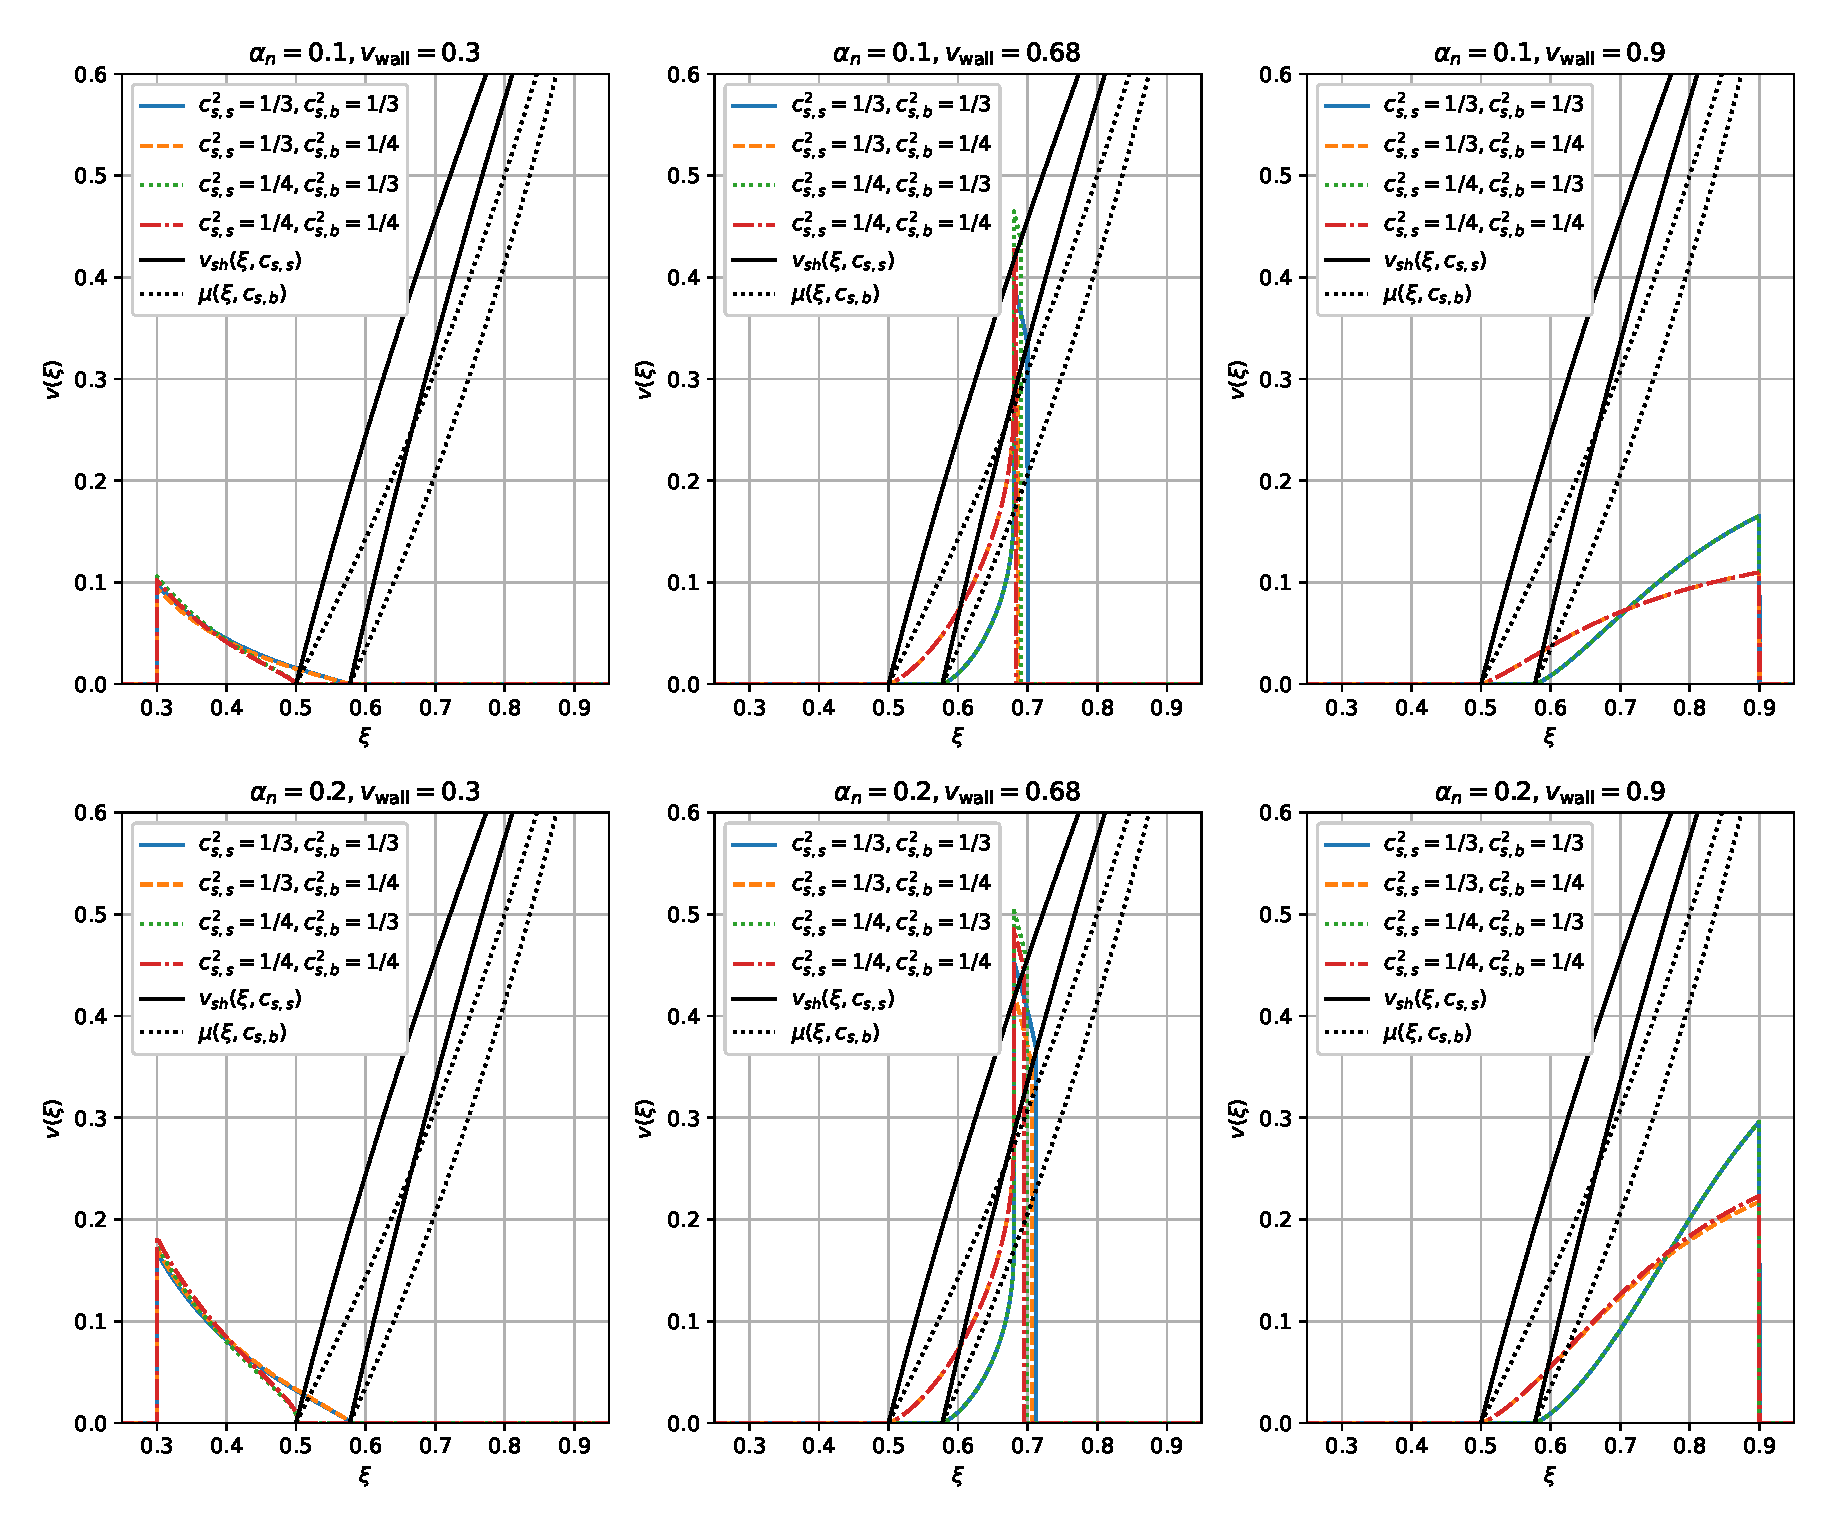
\includegraphics[width=\textwidth]{msc2-python/fig/const_cs_gw_v.eps}
\caption{Self-similar fluid profiles}
\label{fig:fluid_profiles}
\end{figure}

\begin{figure}[ht!]
\centering
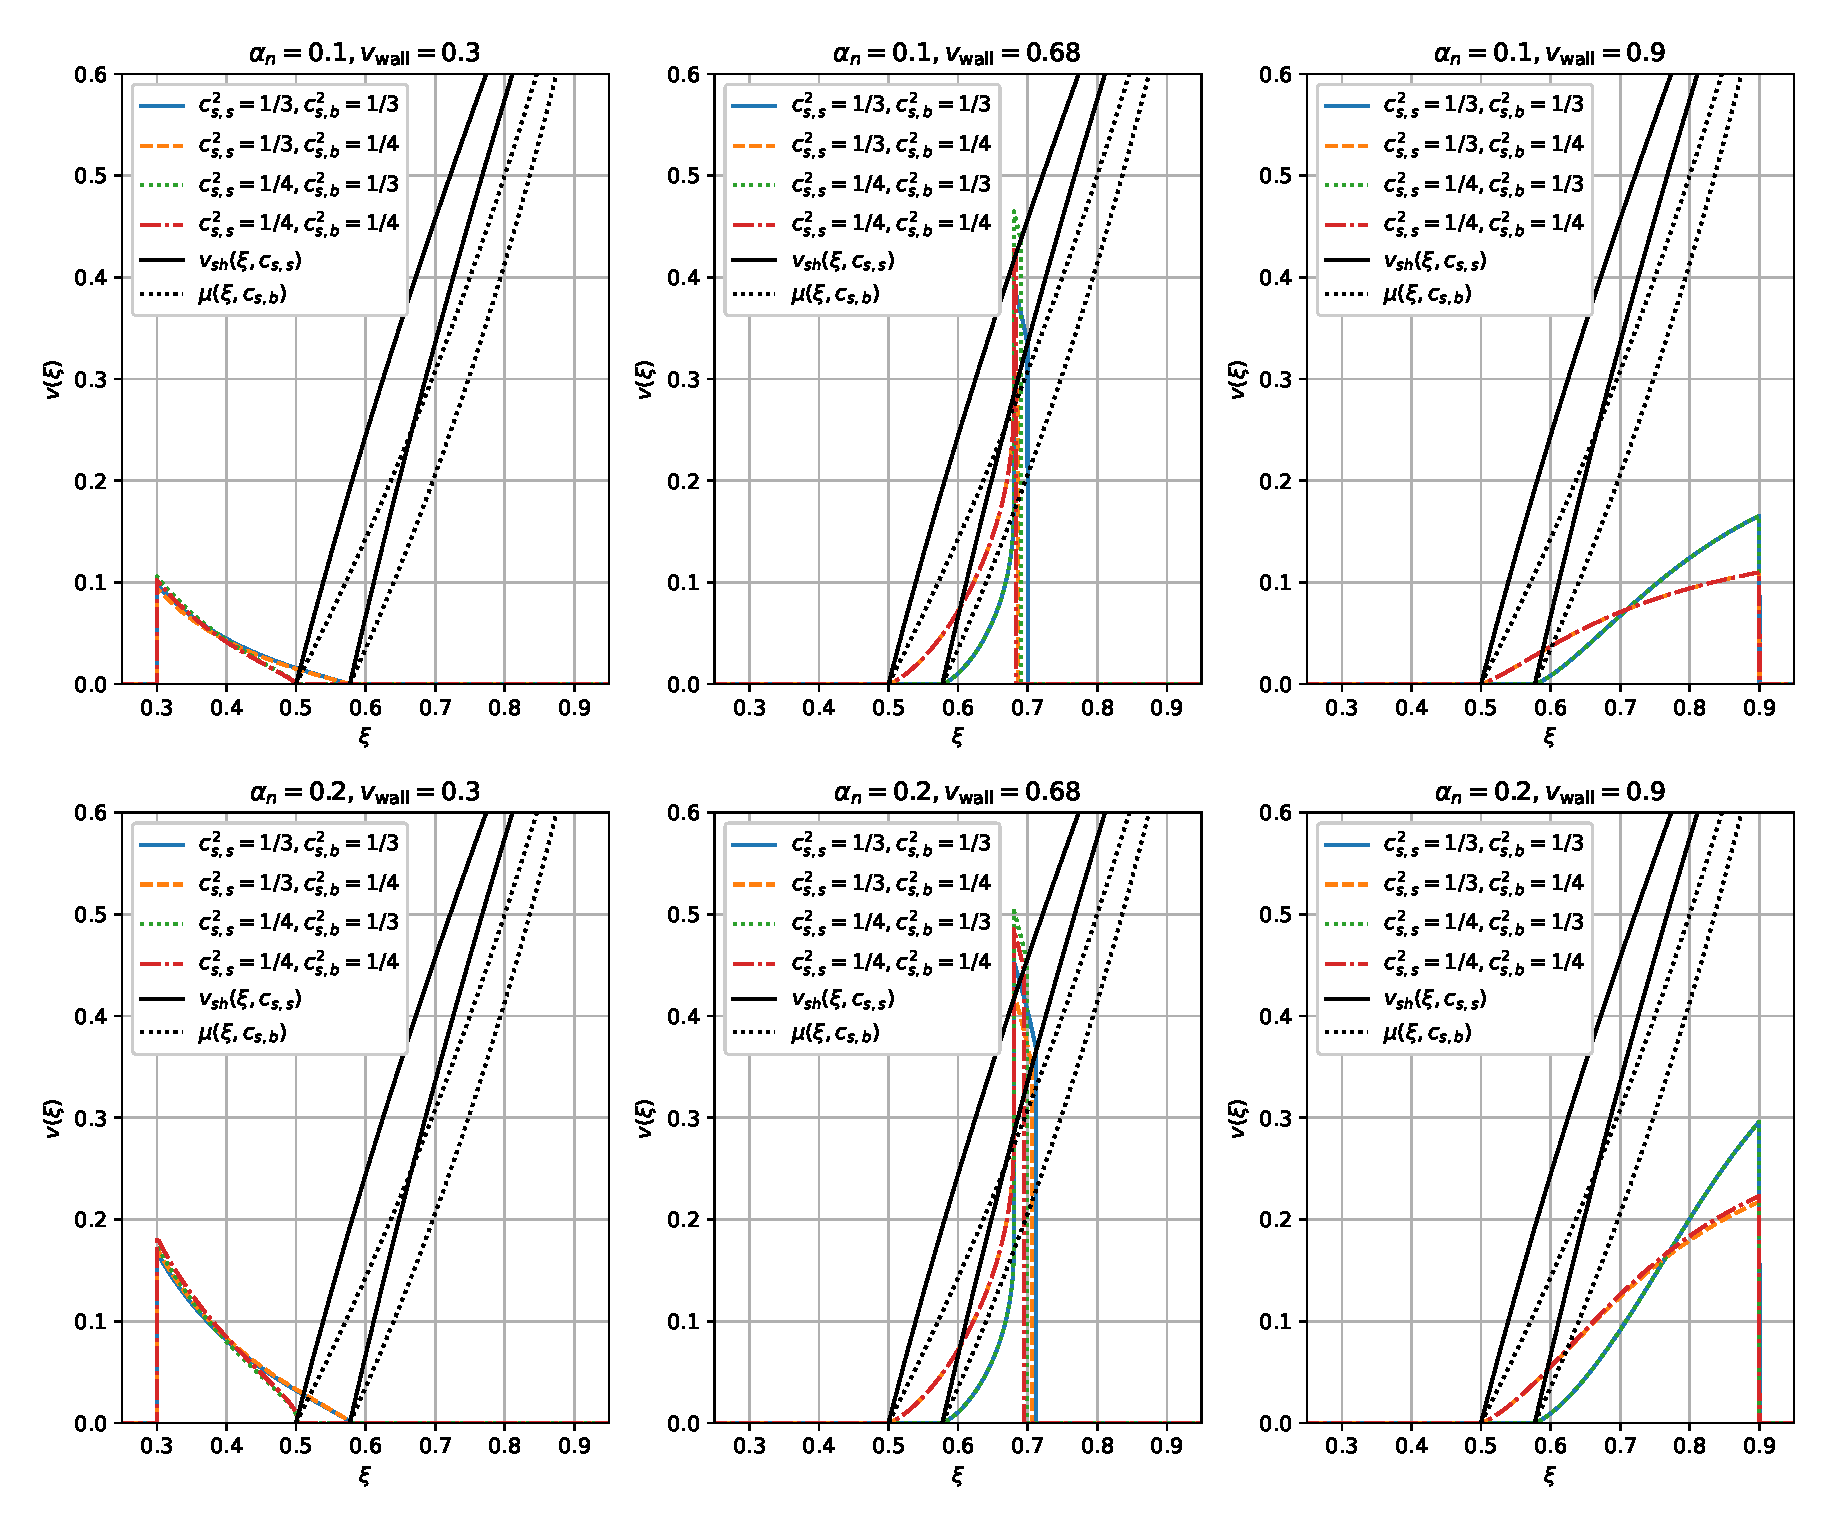
\includegraphics[width=\textwidth]{msc2-python/fig/const_cs_gw_v.eps}
\caption{Gravitational wave power spectra}
\label{fig:gw_spectra}
\end{figure}

\begin{figure}[ht!]
\centering
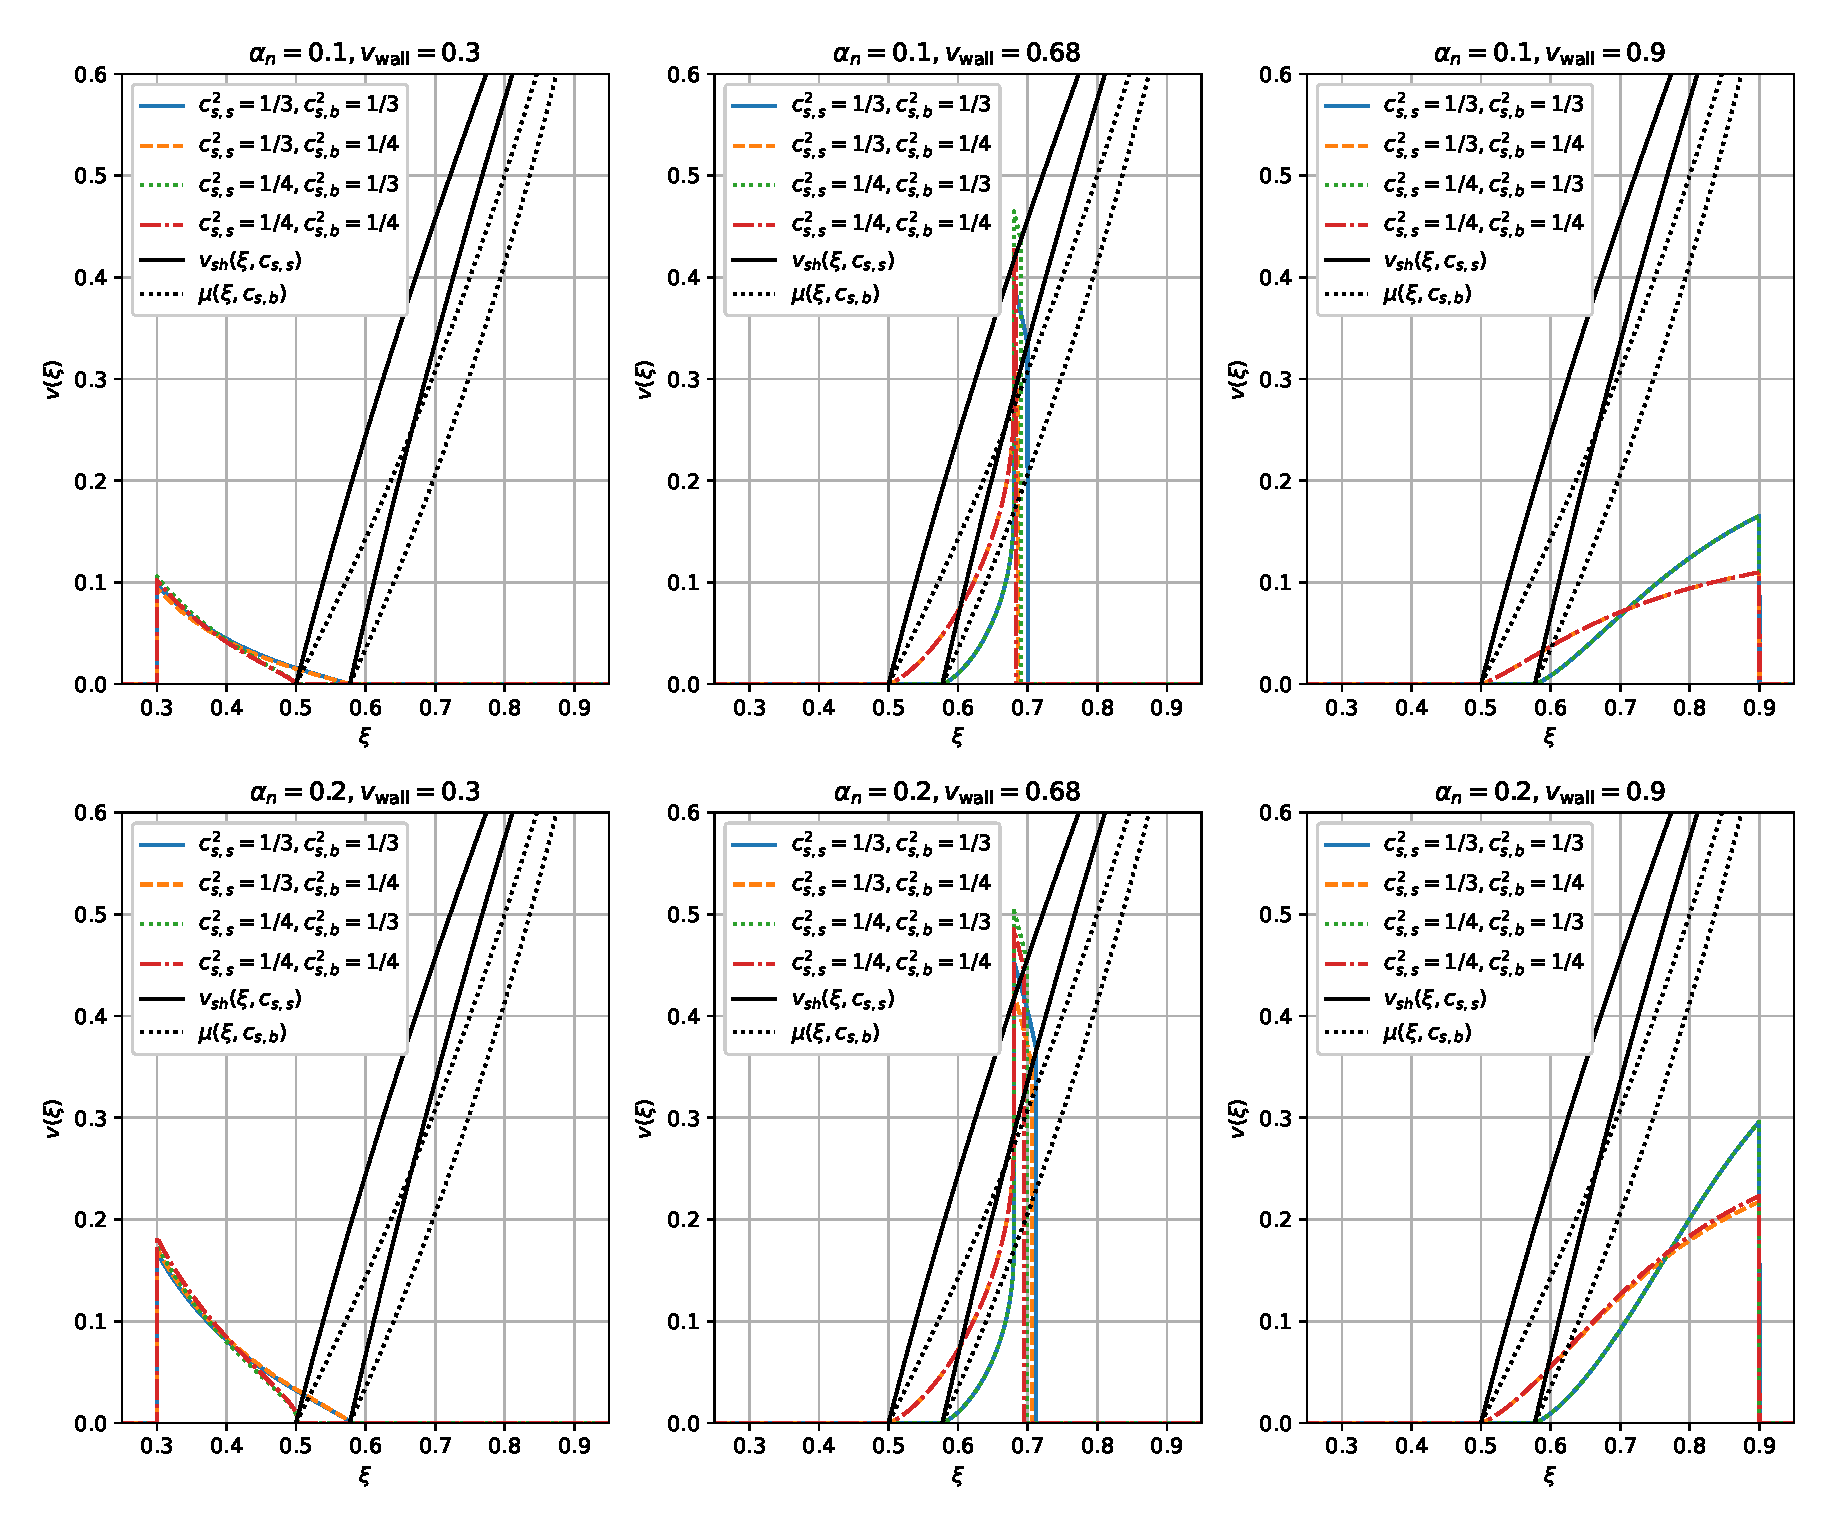
\includegraphics[width=\textwidth]{msc2-python/fig/const_cs_gw_v.eps}
\caption{Scaled gravitational wave power spectra $\Omega_{gw,0}$}
\label{fig:omgw0}
\end{figure}

These figures demonstrate that the sound speed can have a profound effect on the resulting gravitational wave spectrum.
To understand how the sound speed affects the gravitational wave spectrum,
we have to first study the fluid shells of figure \ref{fig:fluid_profiles}.
There are two curves that constrain the shape of the fluid shells.
The solid black curves are the shock velocities $v_{sh}(\xi,c_{s,s})$ that are determined by $c_{s,s}$.
In general the shock velocity is also dependent on $w$, since $c_s = c_s(w,\phi)$,
but in the constant sound speed model the sound speed is independent of the enthalpy,
as it's a constant for each phase.
Therefore we can plot the shock velocities as curves in the 2D plots instead of having to plot them as surfaces as functions of $(\xi,w)$ in a 3D plot.
The dotted black curves are the $\mu(\xi,c_{s,b})$ curves of eq. \eqref{eq:mu} that constrain the maximum fluid velocity inside the bubble.
They are dependent on the choice of $c_{s,b}$.
The $v_{sh}$ curves encounter $v=0$ at $\xi = c_{s,s}$ and the $\mu$ curves at $\xi = c_{s,b}$.

For all solution types, adjusting either of the sound speeds affects the degrees of freedom and therefore the pressure $p$ and enthalpy $w$ for that phase.
This affects the solution of the bubble wall junction conditions of eq. \eqref{eq:junction_condition_1}, \eqref{eq:junction_condition_2} and therefore $v(\xi_\text{wall})$,
which is also the peak of the fluid velocity profile.
This effect can be seen at the top-left figure, where all four fluid shells have different $v(\xi_\text{wall})$.
The change caused by adjusting the sound speed is the most profound for deflagrations when $c_{s,s}$ is decreased below $v_\text{wall}$, as it causes them to become hybrids, and vice versa.
Similarly changing $c_{s,b}$ so that the Chapman-Jouguet speed of \eqref{eq:chapman_jouguet} is decreased below $v_\text{wall}$ converts a hybrid to a detonation, and vice versa.
This can be seen at the top-right figure.

For deflagrations and hybrids, adjusting $c_{s,s}$ affects the location of the shock and therefore the thickness of the fluid shell.
It also affects the ODE group of eq. \eqref{eq:hydro_param1}, \eqref{eq:hydro_param2}, \eqref{eq:hydro_param3} and therefore the shape of the fluid shell in front of the bubble wall.
These effects can be seen at the top-left and bottom-left figures, where the curves with the same $c_{s,s}$ are grouped together.
Correspondingly for hybrids, adjusting $c_{s,b}$ affects $\mu(\xi_\text{wall},c_{s,b})$,
which is the point from which the integration of the detonation-like part of the fluid shell starts.
This can be seen in the two figures at the middle, where the detonation-like tails of the curves with the same $c_{s,b}$ are grouped together.
And for both detonations and hybrids, adjusting $c_{s,b}$ affects the shape of the fluid shell behind the wall.

These differences in the shapes of the fluid shells carry over to the gravitational wave spectra of fig. \ref{fig:gw_spectra} and eventually of the gravitational wave spectra today in fig. \ref{fig:omgw0}.
The sine transformation of eq. \todo{Add equation reference} that converts the fluid shells of fig. \ref{fig:fluid_profiles} to the gravitational wave spectra of \ref{fig:gw_spectra} has the same basic properties as a Fourier transform.
Therefore by comparing the fluid velocity profiles and the gravitational wave spectra we can identify a few general correlations.
The thinner the fluid shell is, the broader the gravitational wave spectrum.
And the higher the fluid velocities are in the fluid shell, the higher is the intensity of the gravitational waves.
Thin shells also have more of the higher frequencies.
These effects can be seen in the case of thin hybrids of the middle and right figures.
Hybrids consist of two sections with significantly differing characteristics.
Therefore the hybrids and especially the thin hybrids with high fluid velocities in front of the wall have a gravitational wave spectrum with two distinct contributions.
This results in a significantly higher gravitational wave spectrum in the higher frequencies resulting in a significantly higher signal-to-noise ratio (SNR),
which distinguishes them from the detonations and deflagrations.
However, regarding hybrids and especially these thin hybrids
it should be noted that the hybrid solutions are very finely tuned, and may not exist in a real fluid.
\cite[p. 5]{gowling_lisa_2021}
Outside the region of the peak, the gravitational wave spectra follow a $k^9$ power law at low $z$,
and $k^{-3}$ at high $z$.

To test the precision and reliability of the results provided by PTtools,
we compared to the results in \cite[fig. 2]{giese_2021},
resulting in figure \ref{fig:kappa_giese}.
It should be noted that the article uses $\kappa_{\bar{\theta}_n}$ of eq. \eqref{eq:kappa_thetabar_n},
which differs from the $\kappa$ defined in eq. \eqref{eq:kappa_omega}.
The colors from blue to gray correspond to $\alpha = 0.01, 0.03, 0.1, 0.3, 1, 3$.
The figures on the left have $\alpha = \alpha_{\bar{\theta}_n}$
and the figures on the right have $\alpha = \alpha_n$.
For each color, the upper line has $c_{s,b}^2 = \frac{1}{3}$ and the lower line $c_{s,b}^2 = \frac{1}{4}$.
The solid lines correspond to $c_{s,s}^2 = \frac{1}{3}$ and the dashed lines correspond to $c_{s,s}^2 = \frac{1}{4}$.

\begin{figure}[ht!]
\centering
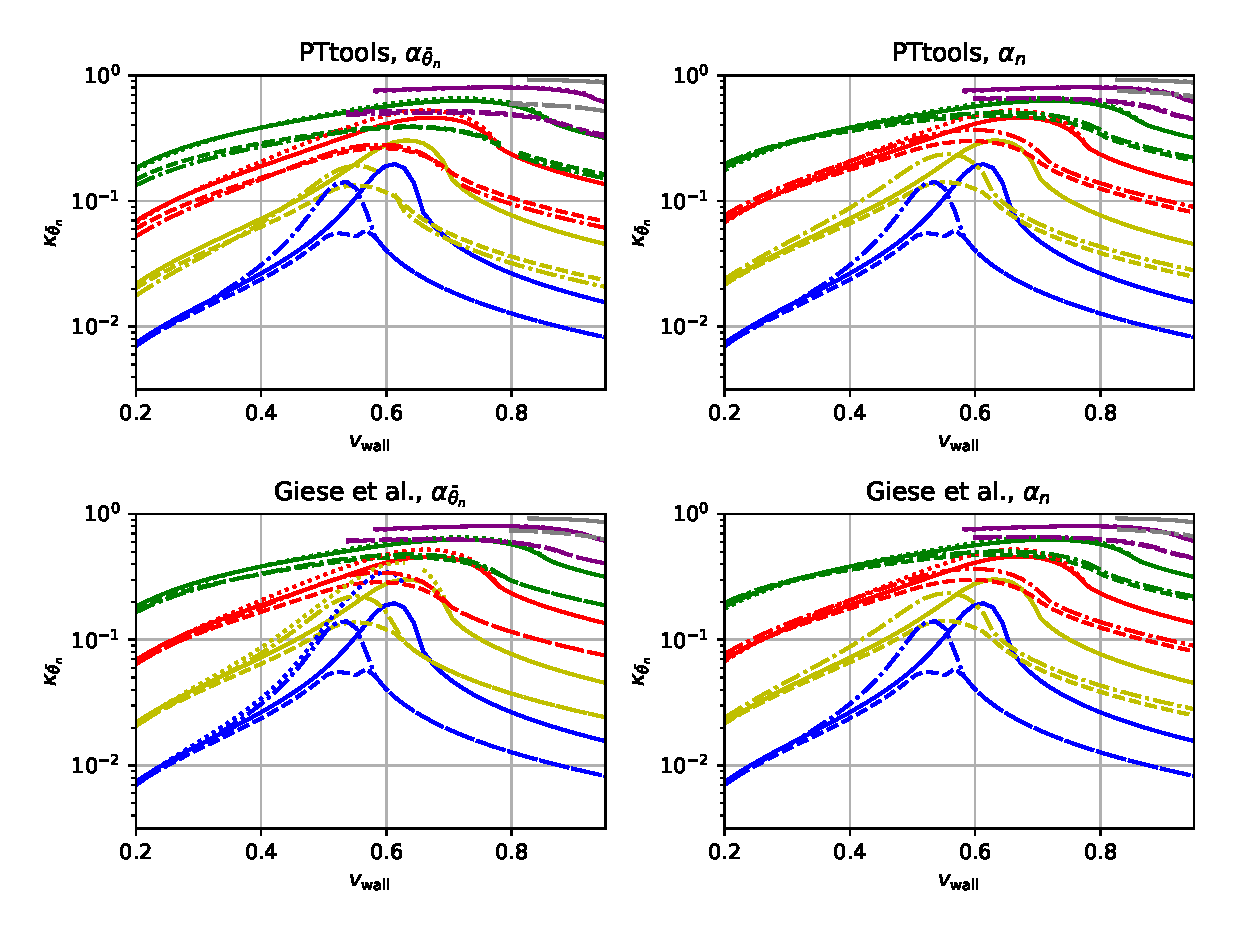
\includegraphics[width=\textwidth]{../pttools/examples/fig/giese_lisa_fig2.eps}
\caption{Comparison of $\kappa_{\bar{\theta}_n}$ values by \cite[fig. 2]{giese_2021} and PTtools}
\label{fig:kappa_giese}
\end{figure}

Comparing the results proved out to be challenging for several reasons.
PTtools operates natively with $\alpha_n$, whereas the Giese code uses $\alpha_{\bar{\theta}_n}$.
Therefore to compare the results, one has to be converted to the other before giving the value to the corresponding code.
There is no known analytical solution for this conversion, and therefore it has to be done numerically.
This may introduce a slight numerical error in $\alpha$ for either one of the solvers.

The Giese code does not check that the input parameter values allow for a physical solution,
and therefore the the parameter region chosen for the figure contains unphysical sections.
For the sound speeds $c_{s,s}^2 = \frac{1}{4}, c_{s,b}^2 = \frac{1}{3}$ the $\alpha = 0.01, 0.03$ values turned out to be below the theoretical minimum
required for a critical temperature to exist.
Therefore the upper dashed blue $\alpha = 0.01$ and yellow $\alpha = 0.03$ lines are missing.
The Giese figures have these solutions, even though they are unphysical.

Nearly all the PTtools figures have a single gap.
This is caused by that particular $\xi_\text{wall}$ value being so near the Chapman-Jouguet speed $v_{CJ}$ of the hybrid-detonation boundary
that the thickness of the fluid shell in front of the is comparable to the minimum step of the ODE solver
and the search step of the shooting algorithm that adjusts the starting point.
This results in the solver being unable to find a solution.
However, it should be noted that this is a pathological special case for the fluid shell solver,
and that for the vast majority of the $(v_\text{wall}, \alpha_n)$ parameter space it works reliably.
Work is being done to improve the solver to work beyond these issues.
The Giese code avoids these issues by using analytical shortcuts specific to the constant sound speed model,
whereas the PTtools solver is intentionally designed to be general so that it will work with more complex models as well.
However, there are also regions in which even the Giese code, as it is shown in an appendix of the article, is not able to find a solution.
Interestingly this curve is present in the figure of the article.
Possible causes include that the code used to generate the figure was different than the one in the appendix,
or that some of the underlying libraries has changed over time.
This is demonstrated by the lack of the dashed blue $\alpha_n = 0.01, c_{s,s}^2 = \frac{1}{4}, c_{s,b}^2 = \frac{1}{3}$ in the bottom-right figure,
and the abrupt end of the same curve in the bottom-left $\alpha_{\bar{\theta}_n}$.

It is also possible that the various validity checks don't capture all the issues at this boundary,
resulting in a slightly wrong result.
This is demonstrated by the solid green $\alpha_n = 0.3, c_{s,s}^2 = \frac{1}{4}, c_{s,b} = \frac{1}{4}$ curve in the top-right figure,
where one of the points deviates from the curve.
These issues continue to be under investigation.

There are also slight differences in the numerical values produced by the solvers.
These are the most visible for the $\alpha_n$ figures, where for high $\xi_\text{wall}$ the effect on changing $c_{s,s}$ has the opposite effect on $\kappa$.
This too continues to be under investigation.
Given that \cites{giese_2020}{giese_2021} are the only known references known by the author regarding the effects of changing the sound speed on the fluid shell profile,
the numerical imprecisions can be either in PTtools or the Giese code, or both.
The development of the code continues.


\chapter{Conclusion}
\label{ch:conclusion}
In this thesis PTtools has been expanded from a compact simulation script based on the bag model
to a comprehensive framework for simulating the fluid velocity profiles of first-order phase transitions in the early universe
and their gravitational wave spectra based on the Sound Shell Model,
including the conversion to the gravitational spectra today.

PTtools was tested with the constant sound speed model due to the availability of reference data by Giese et al. \cite{giese_2021},
and it was shown to work reliably for a broad range of the combinations of the sound speeds $c_{s,s}$ and $c_{s,b}$, the phase transition strength $\alpha_n$ and the wall speed $v_\text{wall}$.
The PTtools fluid velocity profile solver has been updated beyond that of the available references in such a way
that it supports arbitrary particle physics models with a temperature-dependent sound speed $c_s(T,\phi)$,
as long as they provide $V_s(T,\phi), V_b(T,\phi)$ and two of $g_p(T,\phi), g_e(T,\phi), g_s(T,\phi)$ or two of $p(T,\phi), e(T,\phi), s(T,\phi)$, but preferably all three for numerical precision.
This enables the easy integration of models developed by other researchers,
and therefore the comparison of the gravitational wave spectra of these models.
This is also to the author's best knowledge the first time that phase transitions in the early universe have been simulated with temperature-dependent speeds of sound without resorting to time-consuming 3D simulations.

The numerical results of the fluid shell solver have been demonstrated to be consistent with a reference
for a broad range of parameters.
However, some special cases are still challenging.
The most notable of these are very thin hybrid shells near the Chapman-Jouguet speed $v_\text{wall} = v_{CJ}$,
where the thickness of the fluid shell in front of the wall is comparable to the minimum step possible for the ODE solvers.
This limits the precision of the overall solver in these special cases.
However, these special cases compose a very small section of the overall parameter space,
and for the vast majority of the parameter space,
the PTtools solver produces reliable results.

The performance of PTtools is also notable.
The creation of the gravitational wave spectrum today from the phase transition parameters takes less than TODO per bubble on a laptop.
This is in a stark contrast with the 3D hydrodynamic simulations that require the computational power of supercomputers.
This demonstrates that the Sound Shell Model is an essential tool in investigating
the effects of the phase transition parameters on the resulting gravitational wave spectrum.

This master's thesis lays the groundwork for the author's PhD thesis on the topic.
Now there is a framework for determining the gravitational wave spectrum from the phase transition parameters, including temperature-dependent speed of sound.
Determining the parameters of a phase transition from LISA data will require solving the inverse problem: what are the phase transition parameters based on the gravitational wave spectrum?
This will require novel tools such as machine learning or Markov chain Monte Carlo simulations.
There is also potential for integrating PTtools with the existing web-based simulation utility PTPlot to create a comprehensive but easy-to-use utility for researchers to simulate phase transitions with various parameters.
These topics will be investigated in the author's PhD studies.

PTtools will be published as open source soon after the publication of this thesis on GitHub at \cite{pttools}.
This will enable the research community to integrate their various particle physics models,
and to simulate the resulting gravitational wave spectra.
This will provide the LISA simulation pipeline with various waveforms of interest,
and if one of them is eventually found in LISA data,
this will result in a groundbreaking discovery
that will point the direction for the development of particle physics beyond the Standard Model.


\cleardoublepage %fixes the position of the bibliography in bookmarks
\phantomsection

\addcontentsline{toc}{chapter}{\bibname} % This lines adds the bibliography to the ToC
% \bibliographystyle{abbrv} % numbering alphabetic order
% \bibliography{bibliography}

% \printbibliography[heading=bibintoc]
\printbibliography

% \begin{appendices}

% \end{appendices}


\end{document}

% This is for ensuring that arXiv runs pdflatex at least 4 times.
% https://trevorcampbell.me/html/arxiv.html
\typeout{get arXiv to do 4 passes: Label(s) may have changed. Rerun}
